\documentclass[a4paper, 50pt, twoside]{article}
\usepackage[italian]{babel}
\usepackage[a4paper, top=2cm, bottom=2cm, left=3cm, right=3cm]{geometry}
\usepackage{graphicx}
\graphicspath{{immagini/}}
\usepackage{chngcntr}
\counterwithin{figure}{section}
\usepackage{braket}
\usepackage{amsmath}
\usepackage{fancyhdr}
\usepackage{xcolor}
\usepackage{listings}
\usepackage{pxfonts}
\pagestyle{fancy}
\lfoot{EasyVersity}

\definecolor{grigio}{rgb}{0.85,0.85,0.85}
\lstset{
language = Java,
basicstyle = \ttfamily \small,
keywordstyle = \bfseries,
numbers = left,
backgroundcolor = \color{grigio},
showstringspaces = false,
tabsize = 2
}

\begin{document}


\title{EasyVersity}
\date{Settembre, 2019}
\author{Tomassini Danilo \\ Cappella Simone \\ Mannini Luca \\ \\ Ingegneria Informatica e dell'Automazione}
\maketitle
\vspace*{\fill}
\begin{figure}[h!]
	\centering
	
\includegraphics[width=\linewidth]{copertina4.jpg}
	\label {fig::copertina}
\end{figure}
\vspace*{\fill}

\newpage
\tableofcontents{}

\newpage
\section{Obbiettivi}
EasyVersity rappresenta uno strumento di supporto per lo studente.

Permette di gestire:
\begin{itemize}
\item \textbf{Orario:} salva l'orario delle lezioni nella tua applicazione per consultarlo quando vuoi.
\item \textbf{Archivio appunti locale:} da la possibilità di salvare appunti raggruppandoli per materia, indicando titolo e data si può contestualizzare al meglio l'appunto in questione.
\item \textbf{Condivisione appunti:} rende possibile la condivisione ed il download degli appunti.
\item \textbf{Impostazioni:} da qui si possono cambiare informazioni come username e password, eprendere visione di info "about us".
\end{itemize}

\section{Funzionalità}
Avviata l'applicazione ci si trova davani alla \textbf{First activity}; qui si può scegliere di effettuare il login o registrarsi. Una volta effettuato il login si può accedere al menù principale che prevede 4 scelte:
\begin{itemize}
\item \textbf{Orario.}
\item \textbf{I miei appunti.}
\item \textbf{Appunti condivisi.}
\item \textbf{Impostazioni.}
\end{itemize}
\begin{figure}[!h]
	\centering
	{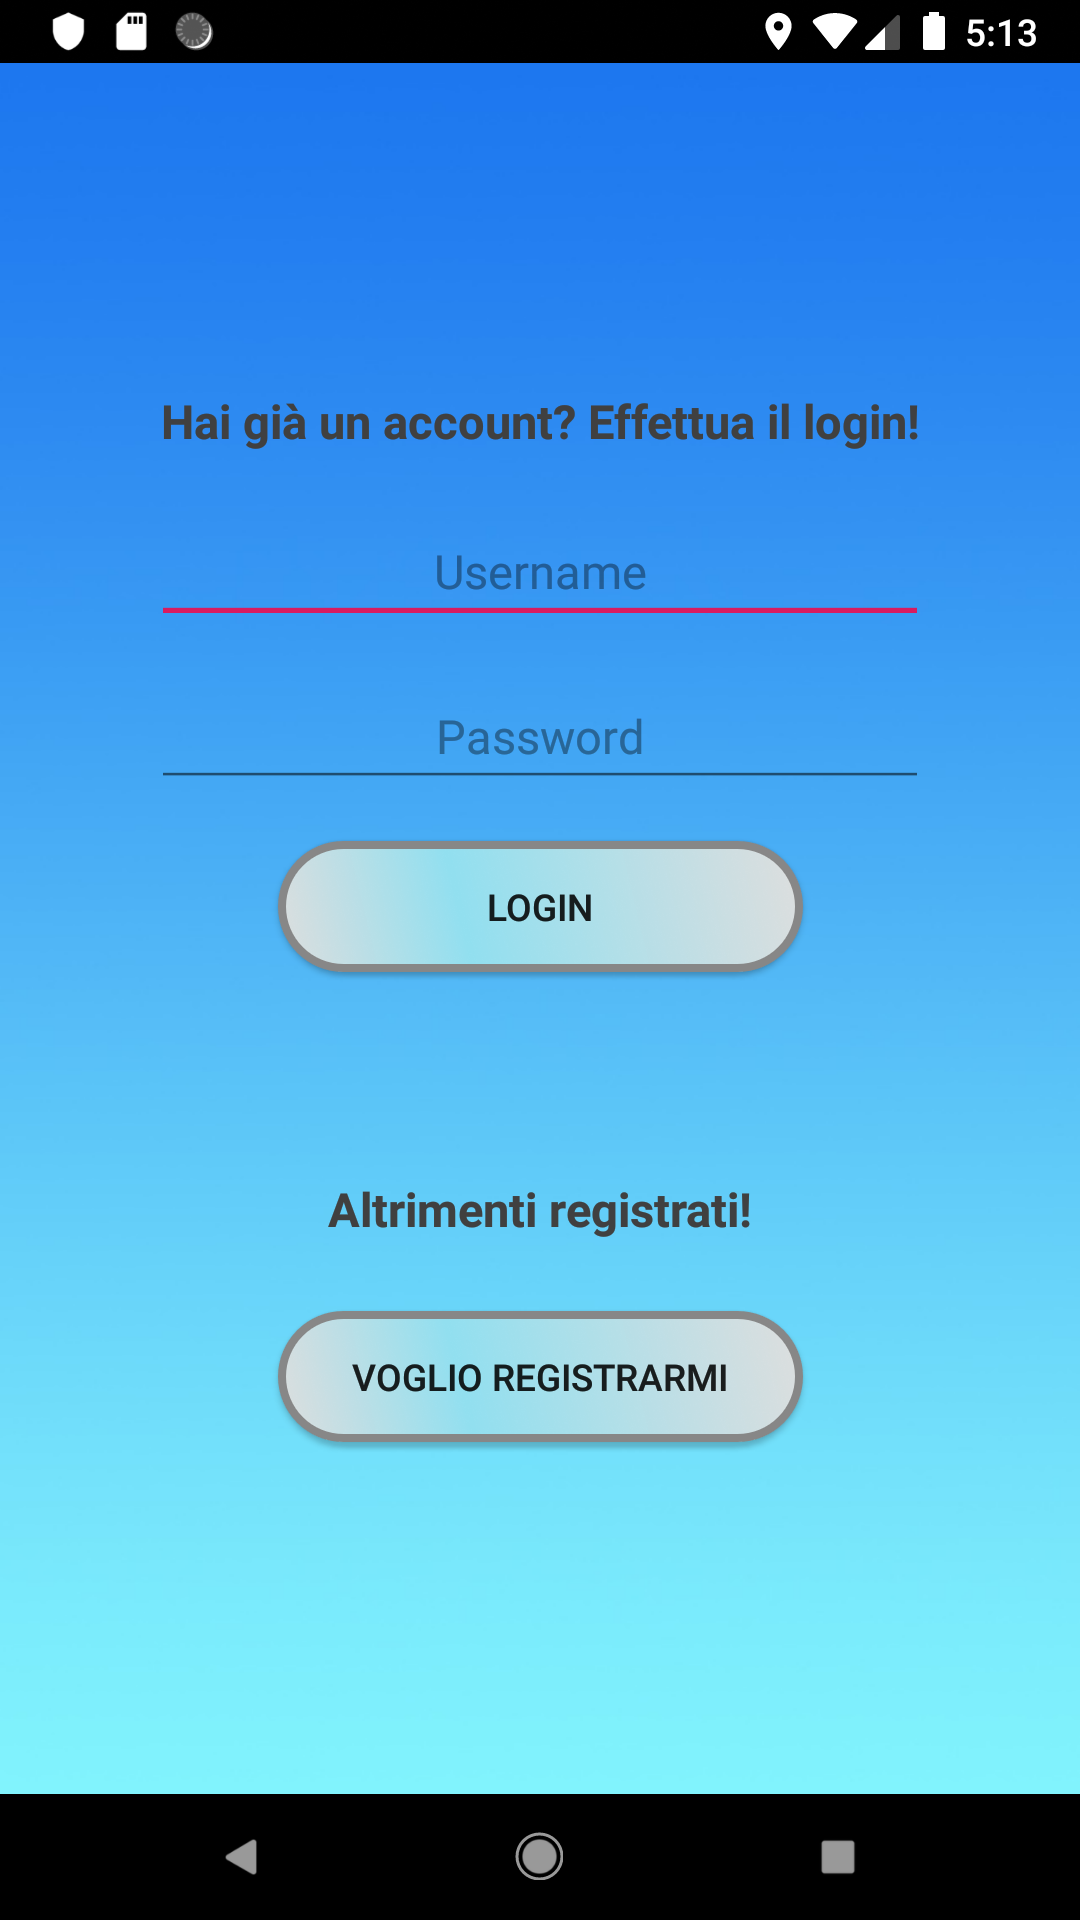
\includegraphics[width=.30\textwidth]{login}} \quad
	{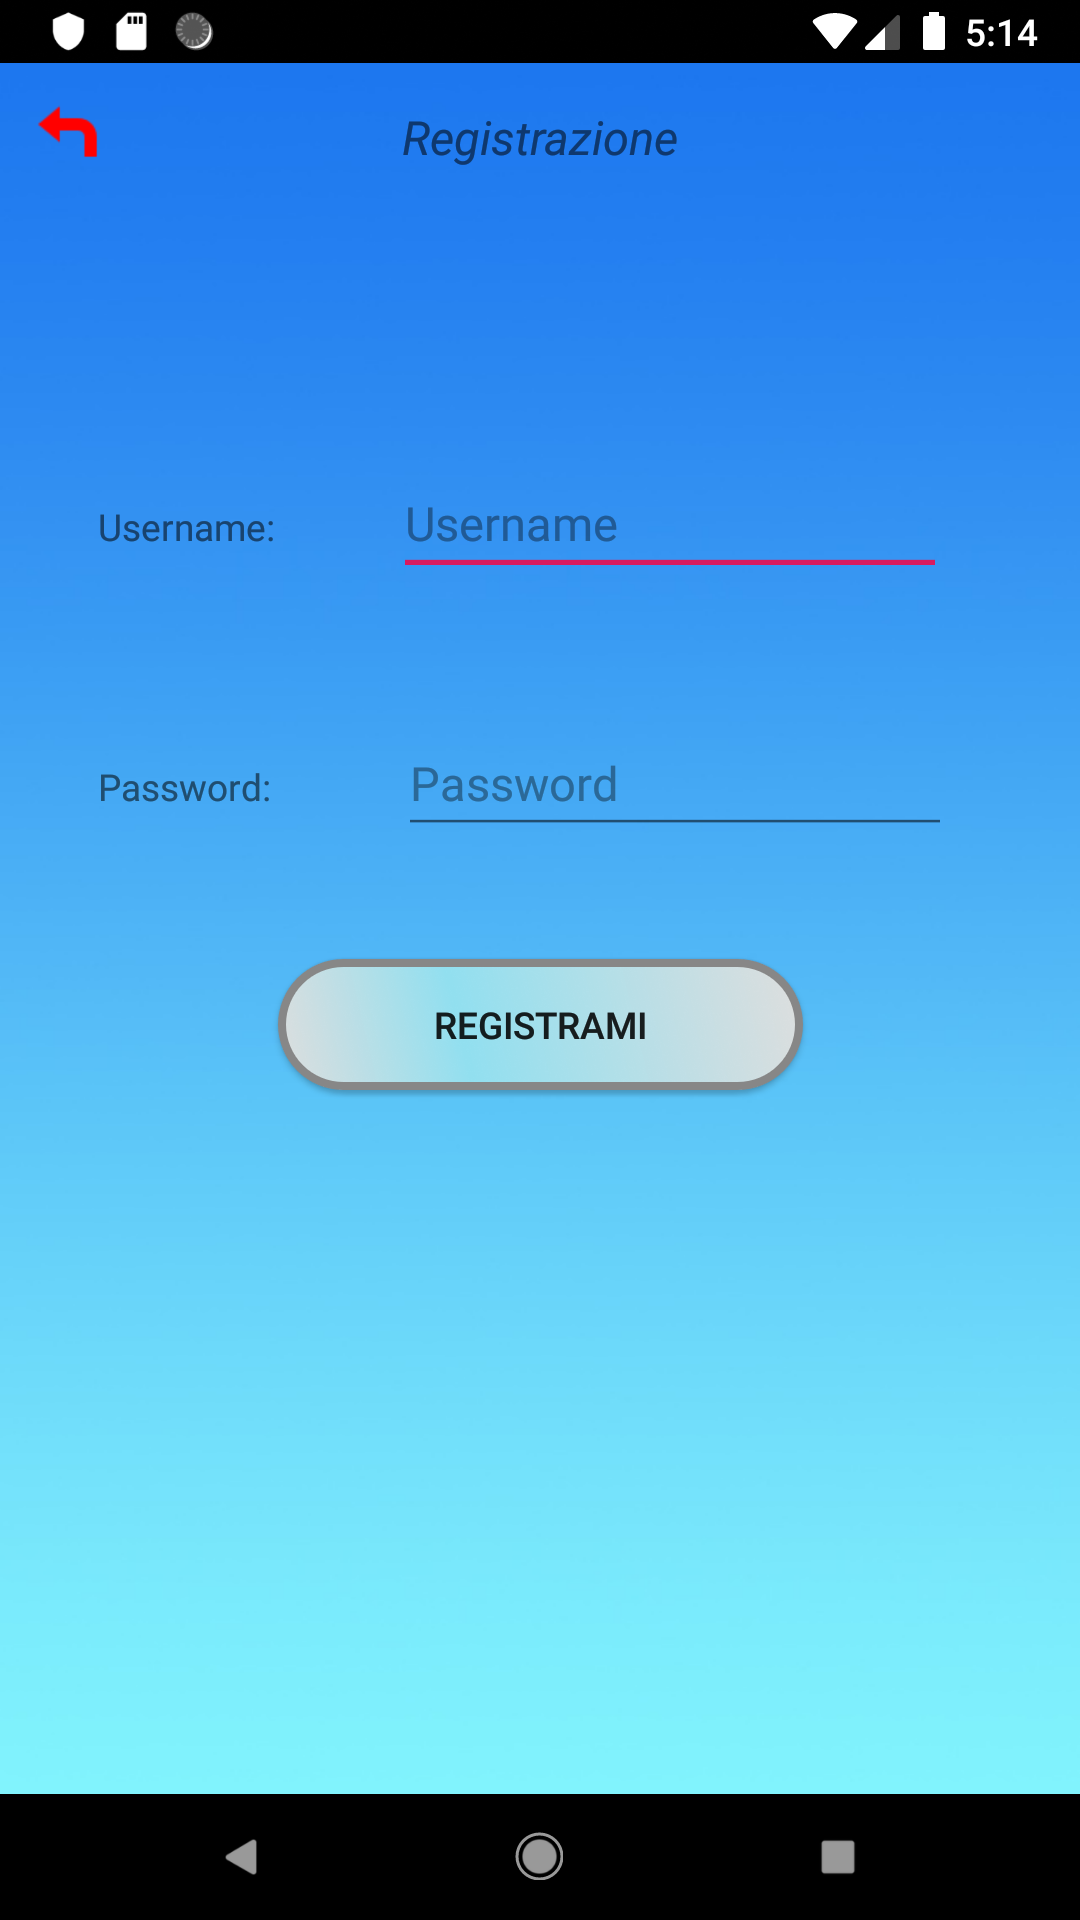
\includegraphics[width=.30\textwidth]{registrazione}} \quad
	{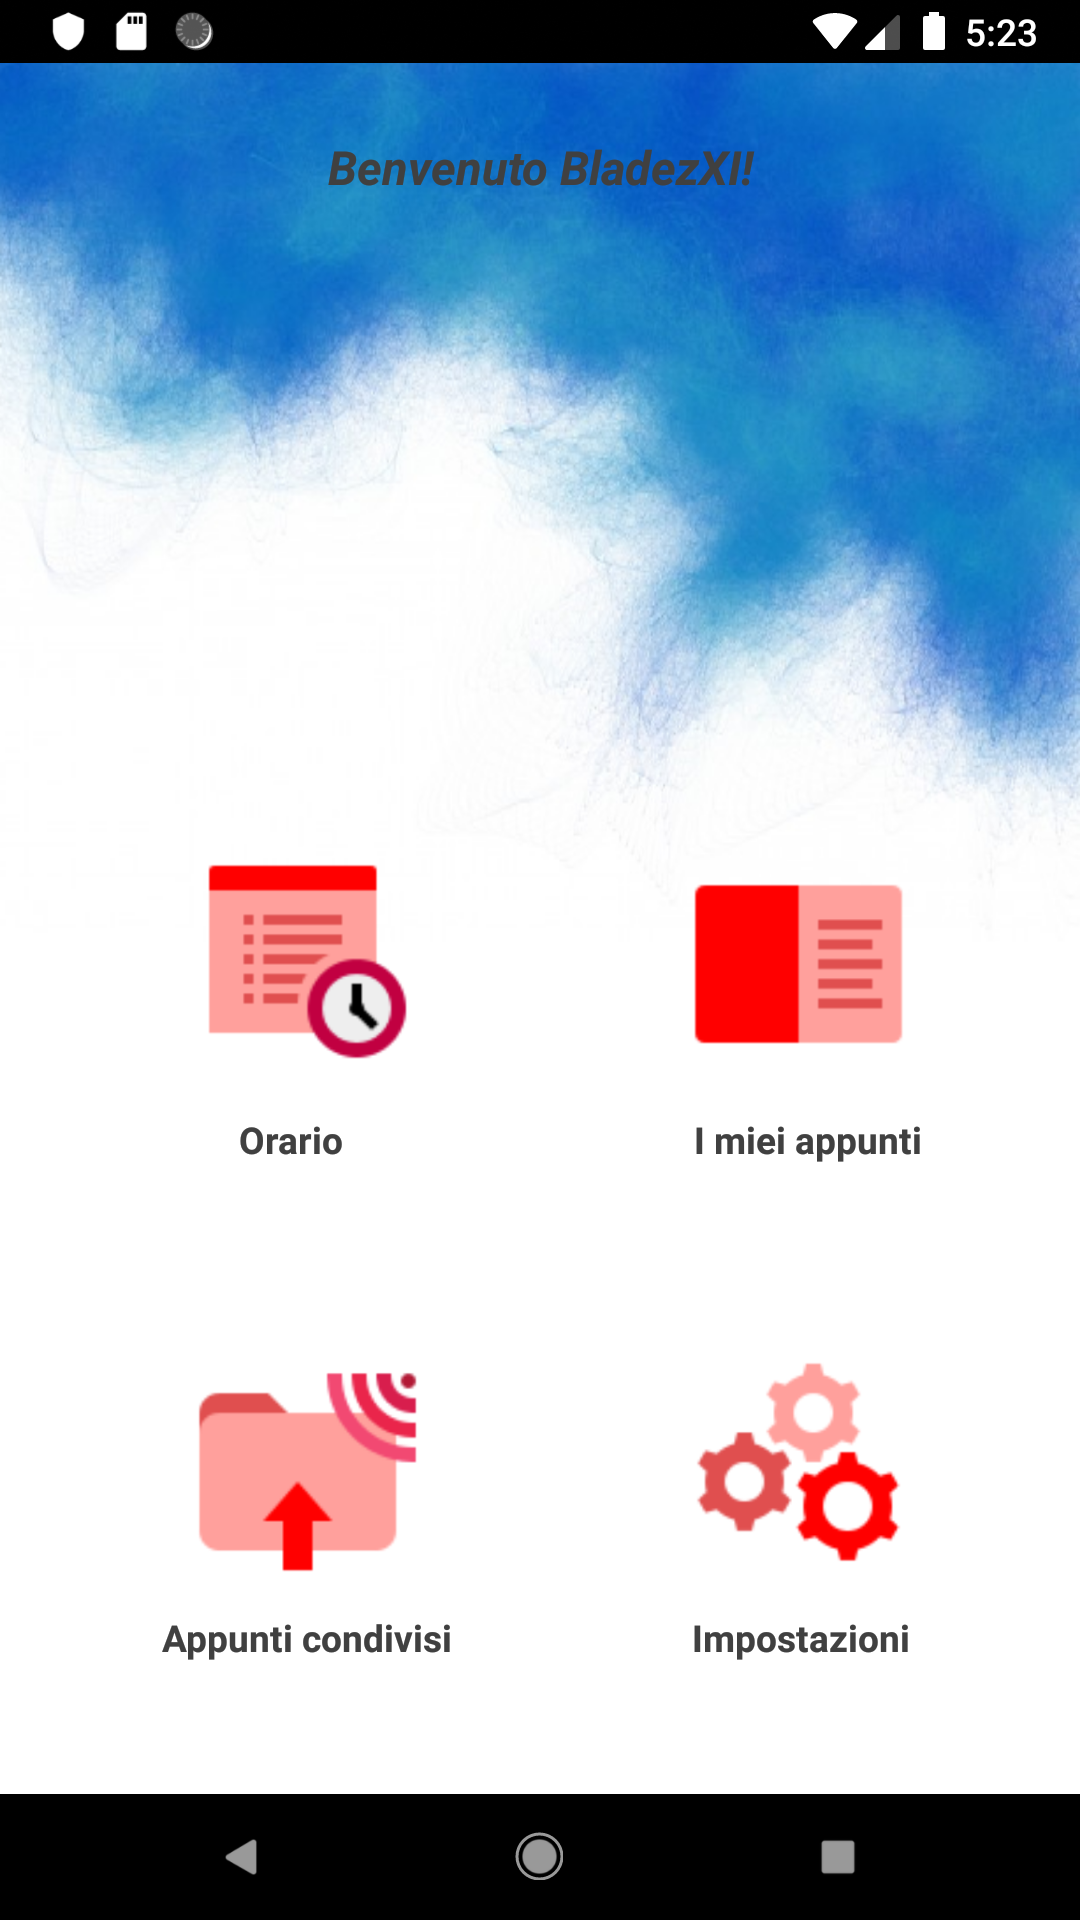
\includegraphics[width=.30\textwidth]{menu}}
	\caption{\small Schermata Login, Registrazione e Menu principale.}
\end{figure}

\newpage
\subsection{Orario}
Aperto l'orario ci si trova di fronte alla tabella relativa al giorno corrente; con la bottom navbar si può scegliere il giorno su cui andare ad agire.
Premendo nel campo \textbf{materia}, relativo all'ora di interesse si può inserire la materia in tabella, si accede, infatti, ad una lista predefinita di materie (questa può essere estesa scegliendo di inserirne una manualmente con il bottone "altro"). Scelta la materia viene visualizzata una finestra di dialogo che permette di inserire l'aula in cui si svolgerà la lezione e la durata della stessa.
\begin{figure}[!h]
	\centering
	{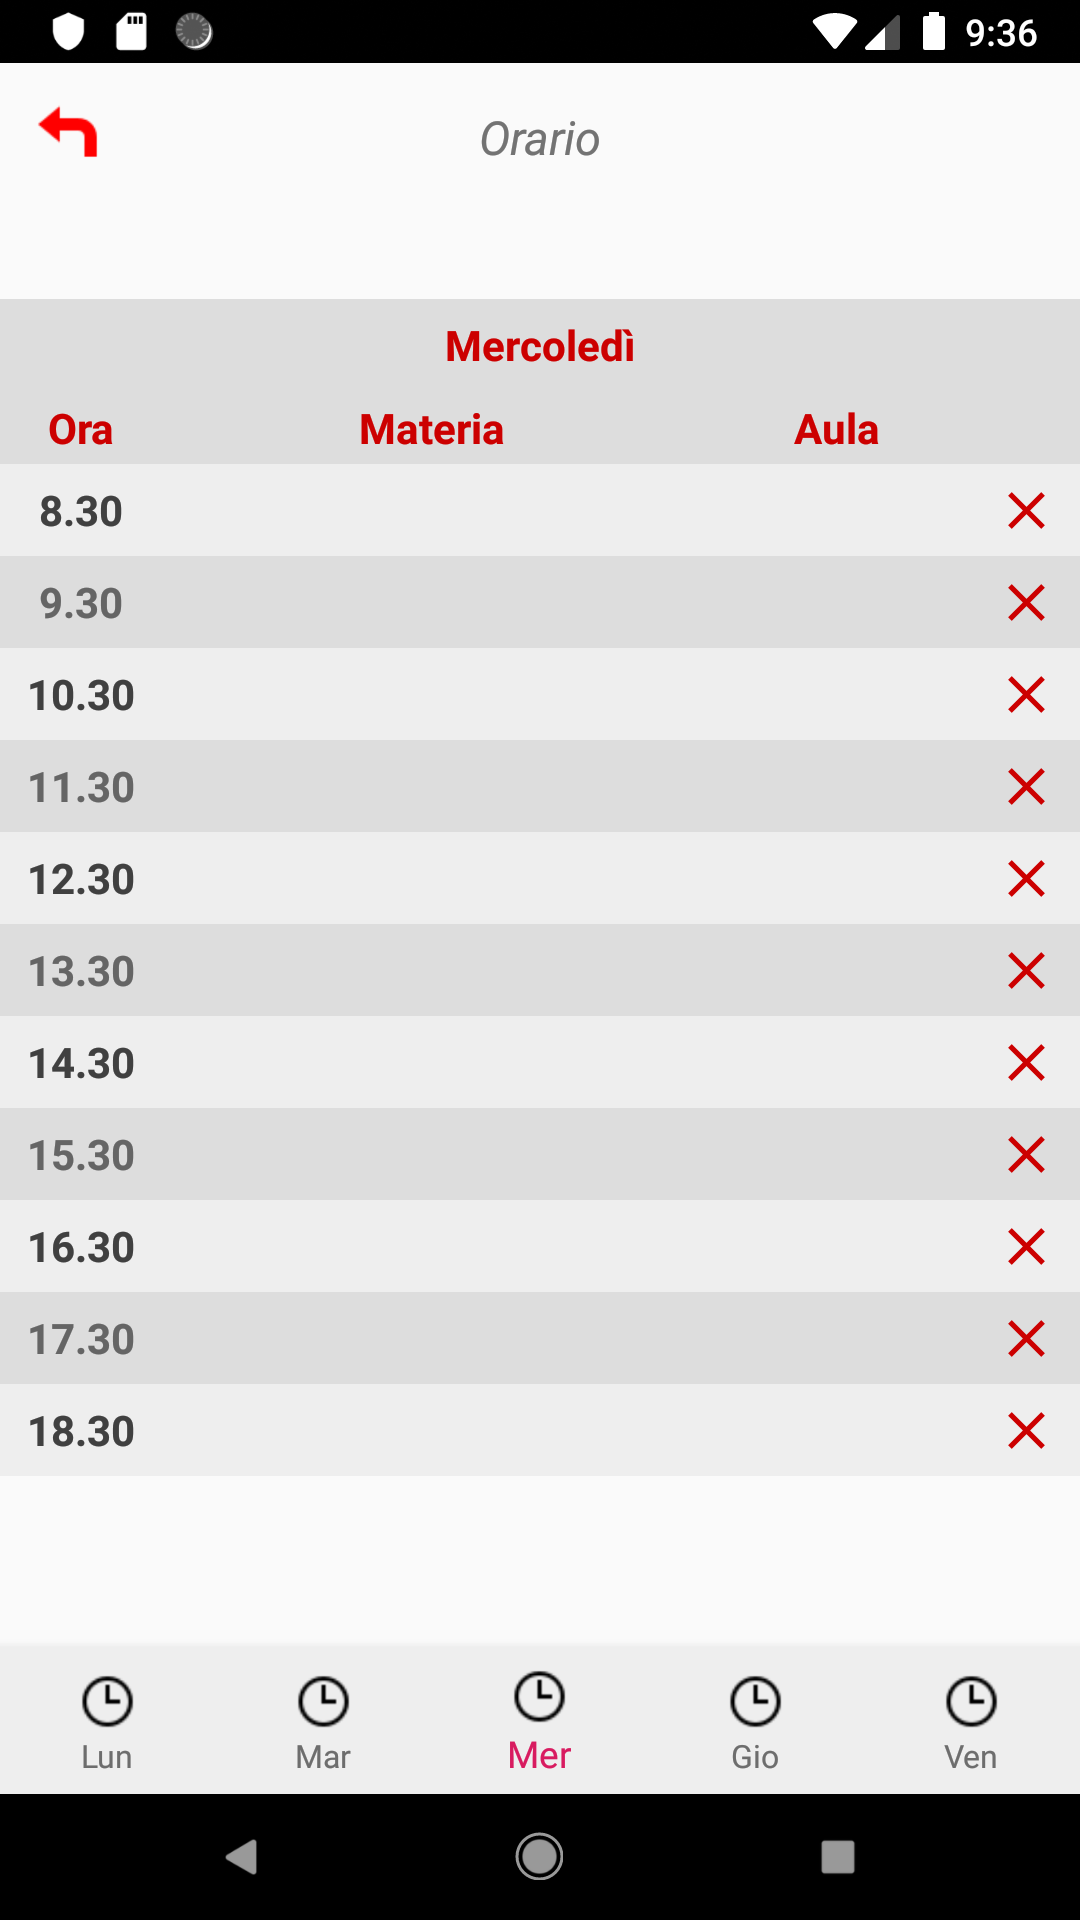
\includegraphics[width=.30\textwidth]{orario}} \quad
	{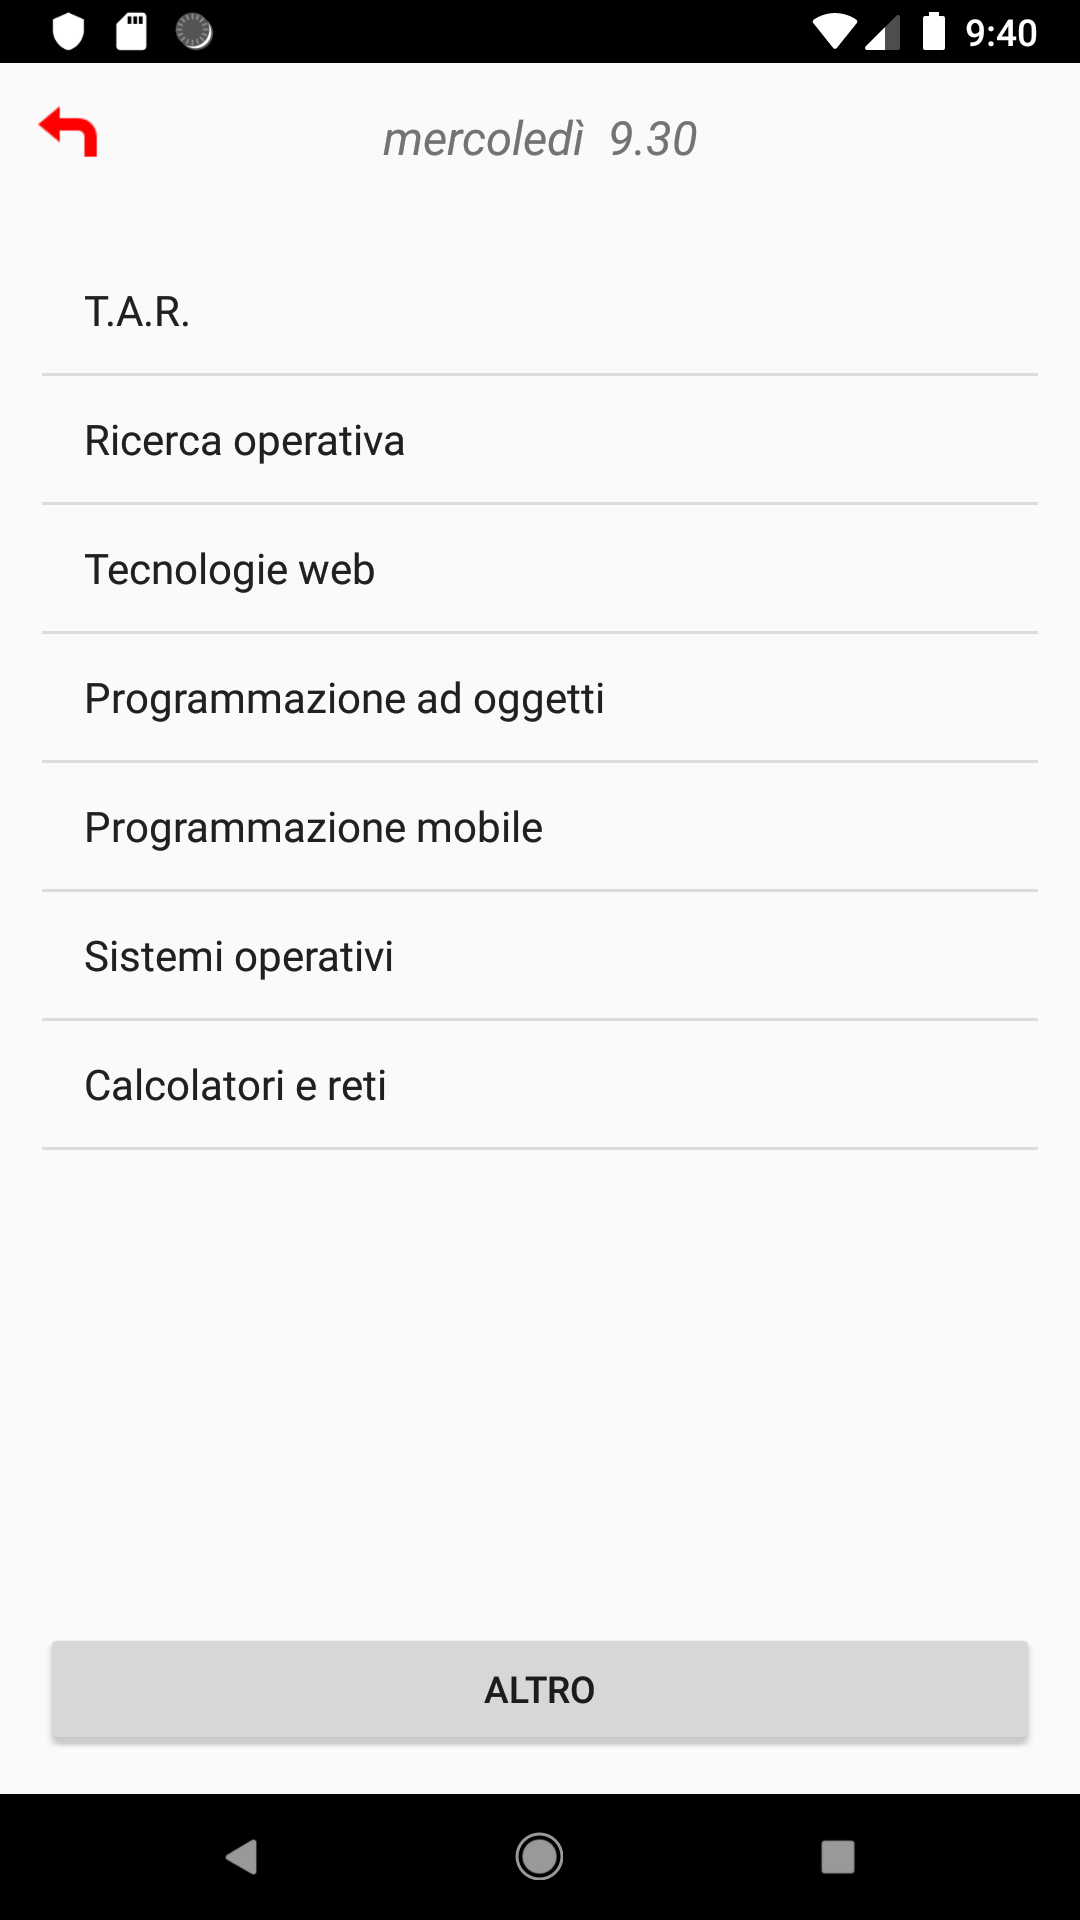
\includegraphics[width=.30\textwidth]{orario_scelta_materia}}\quad
	{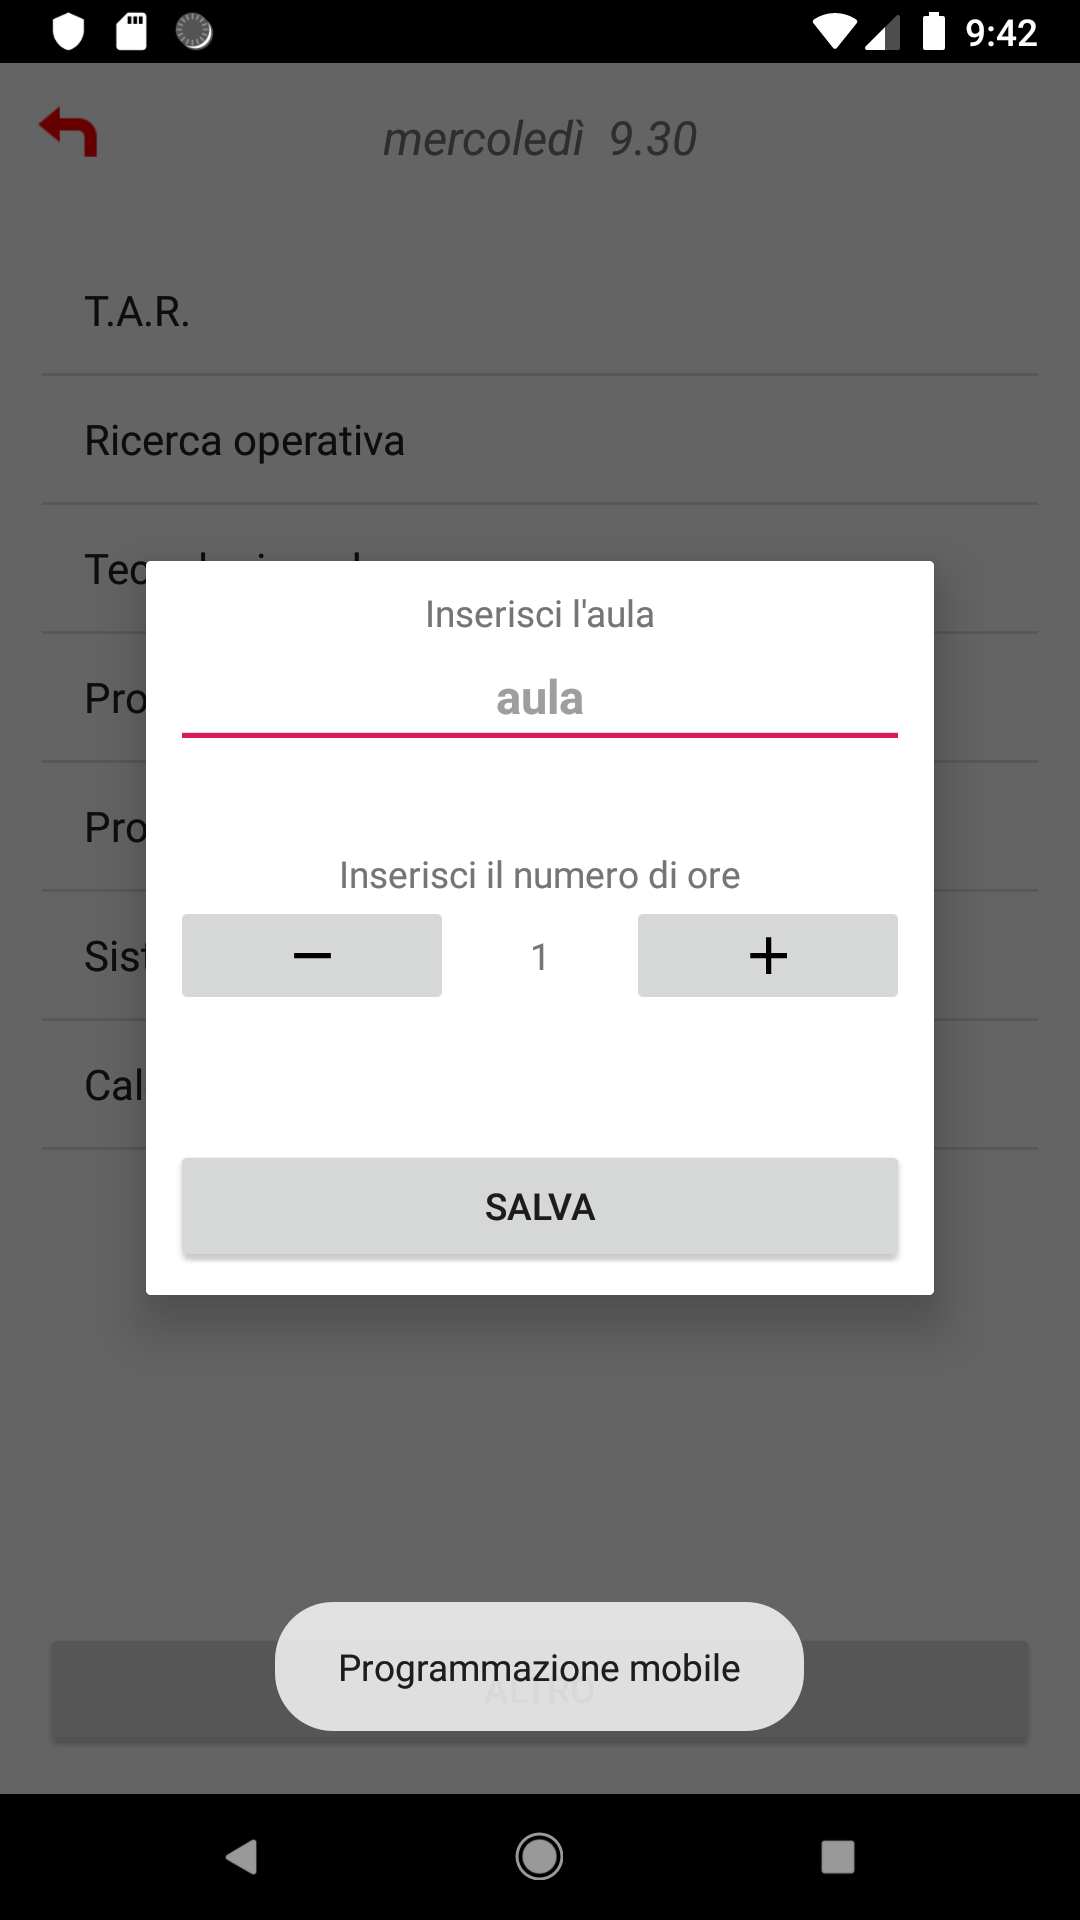
\includegraphics[width=.30\textwidth]{orario_inserimento}}
	\caption{\small Orario.}
\end{figure}

Salvata la materia nell'orario questa viene salvata nel database e inserita in una lista nella sezione \textbf{i miei appunti}.

\subsection{I miei appunti}
In questa sezione abbiamo accesso alla lista di tutte le materie salvate nel database. Abbiamo la possibilità di aggiungerne altre a piacimento o eliminarle inserendo il nome esatto della materia.

\begin{figure}[!h]
	\centering
	{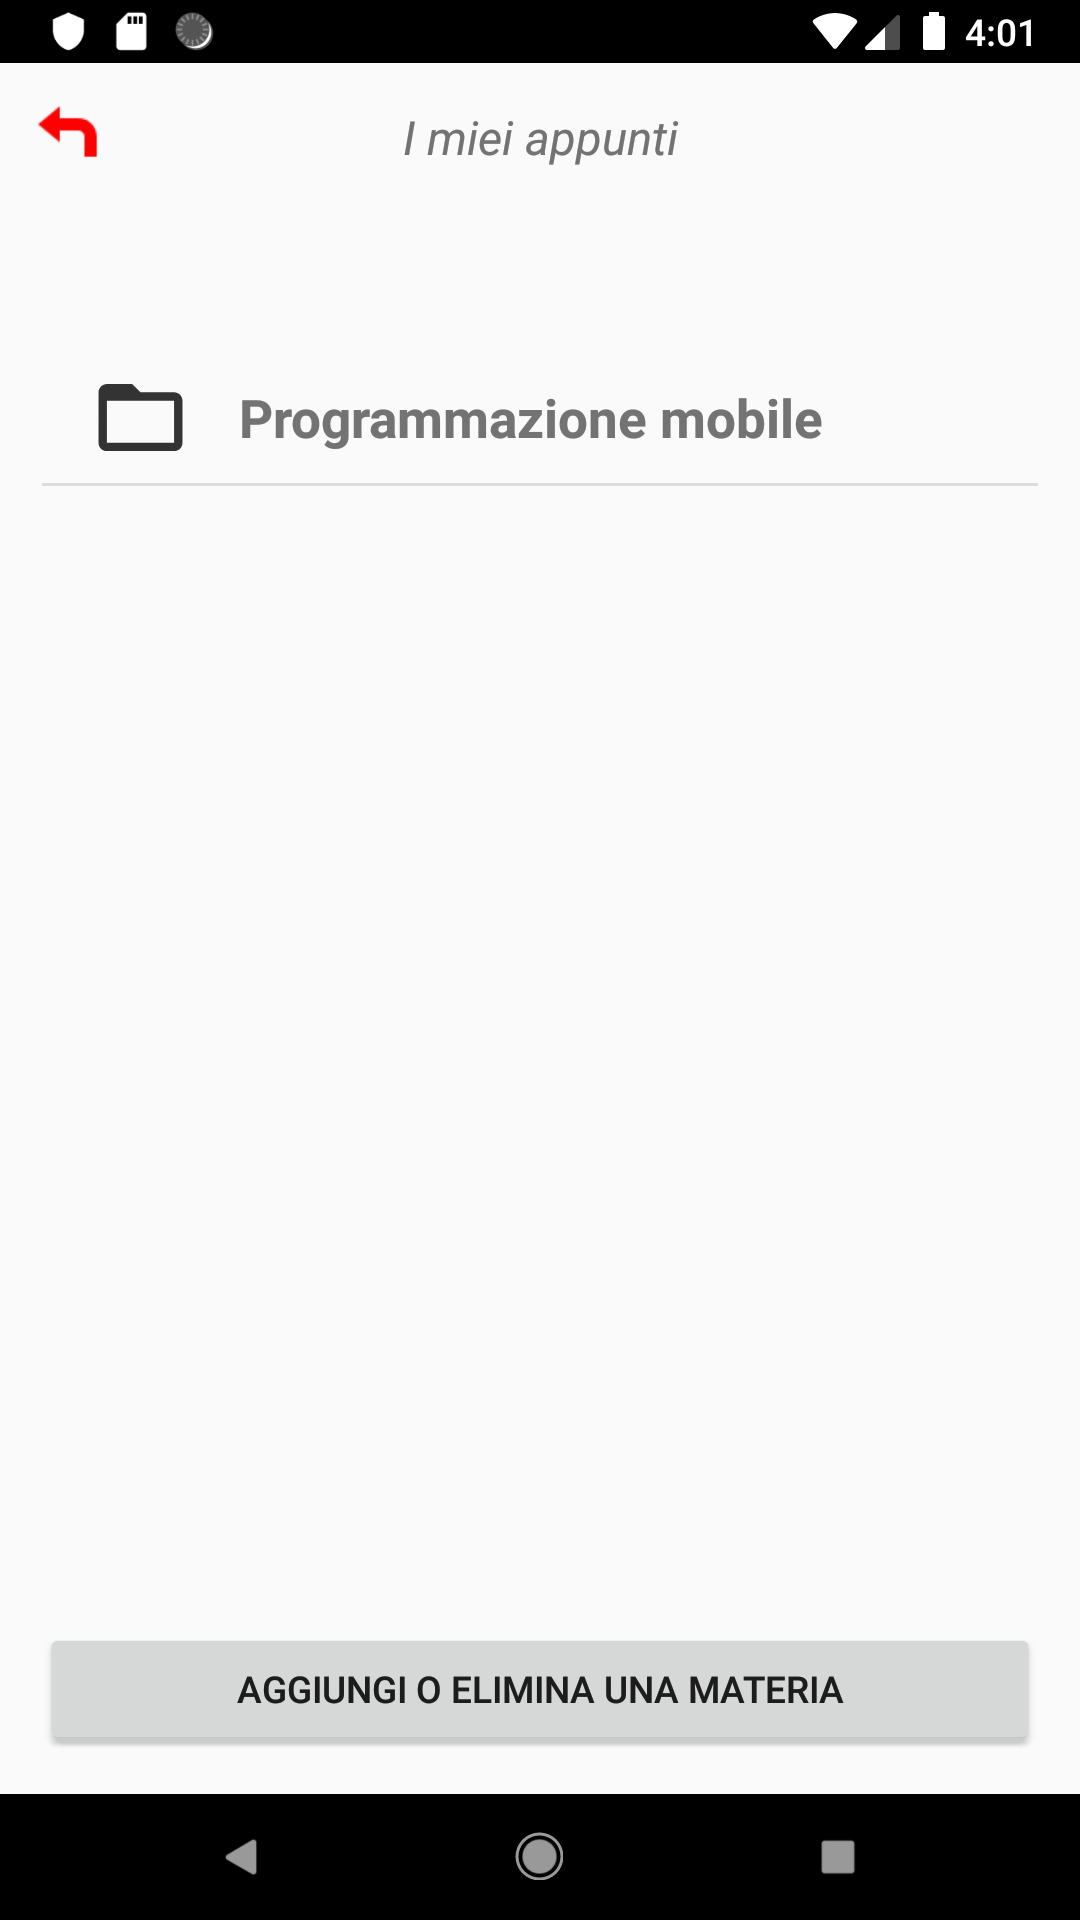
\includegraphics[width=.30\textwidth]{miei_appunti_lista_materie}} \quad
	{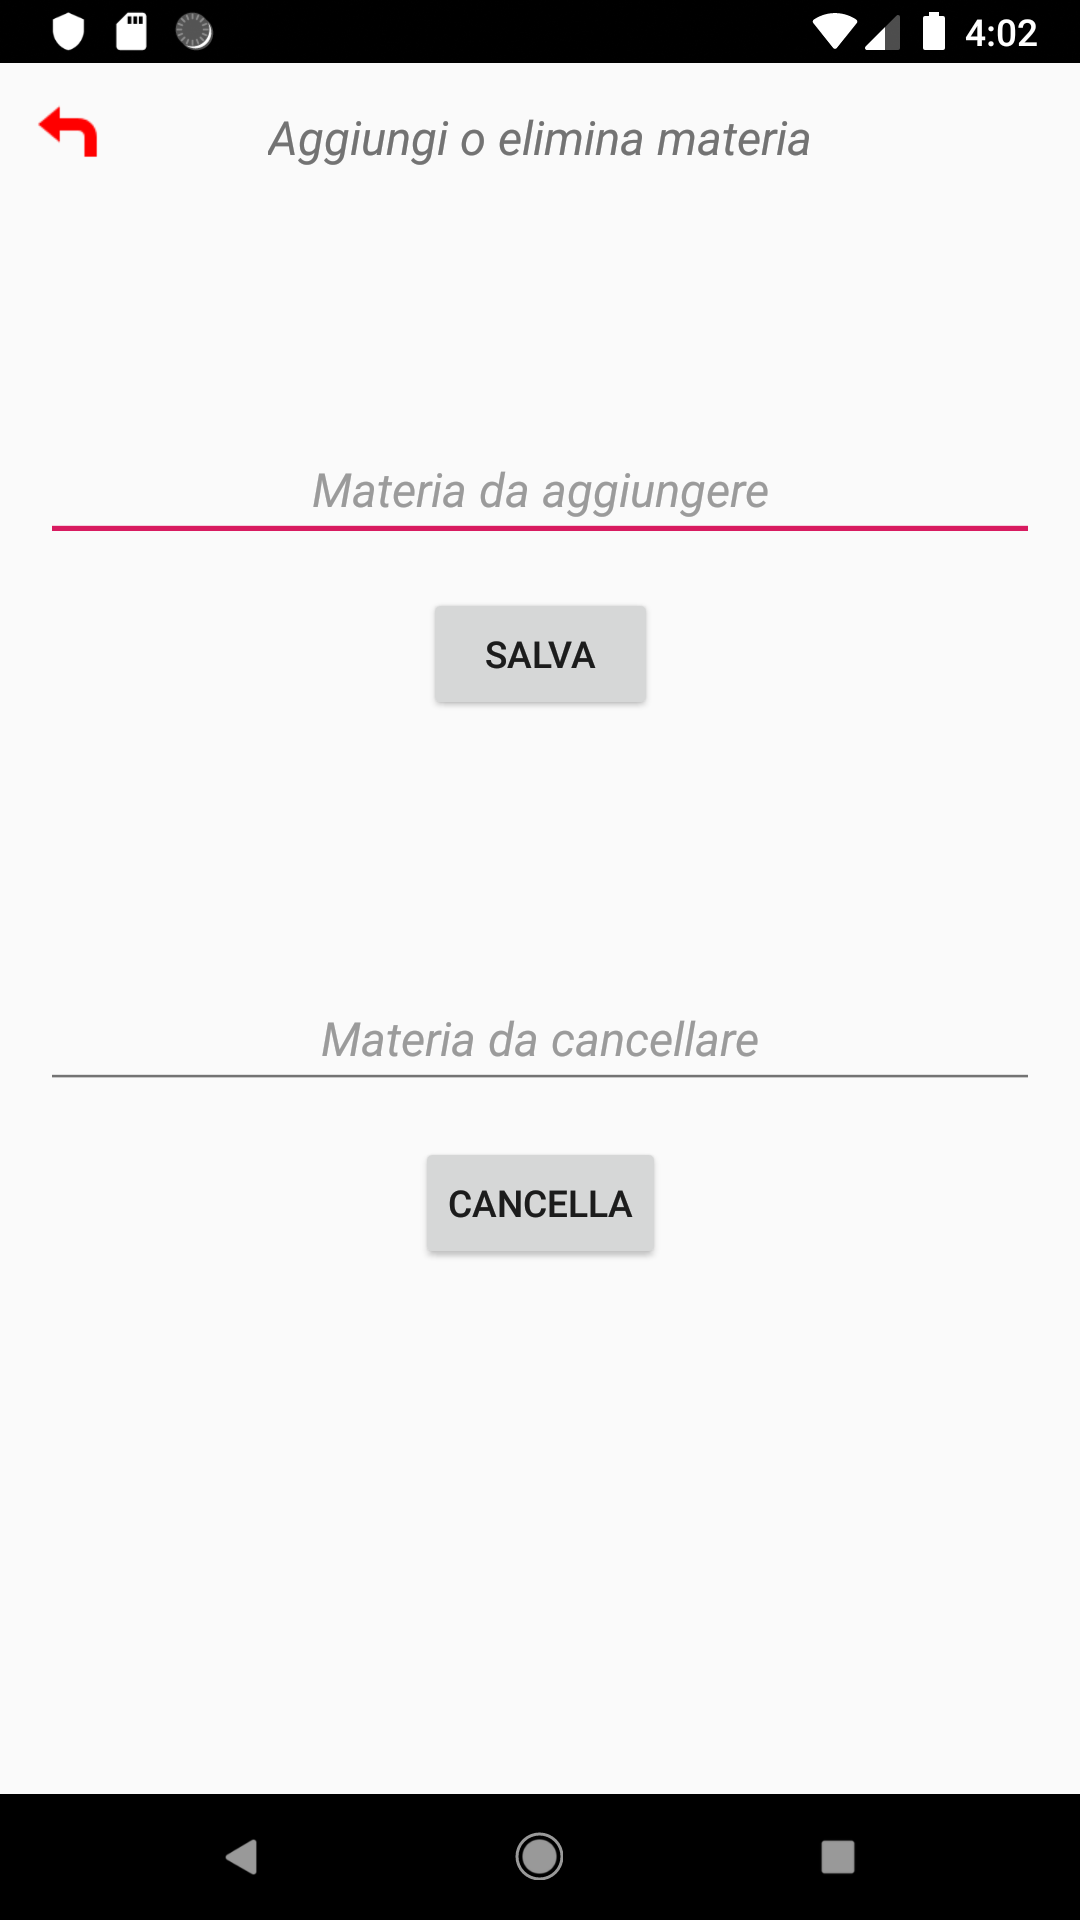
\includegraphics[width=.30\textwidth]{miei_appunti_aggiungi_materia}} \quad
	{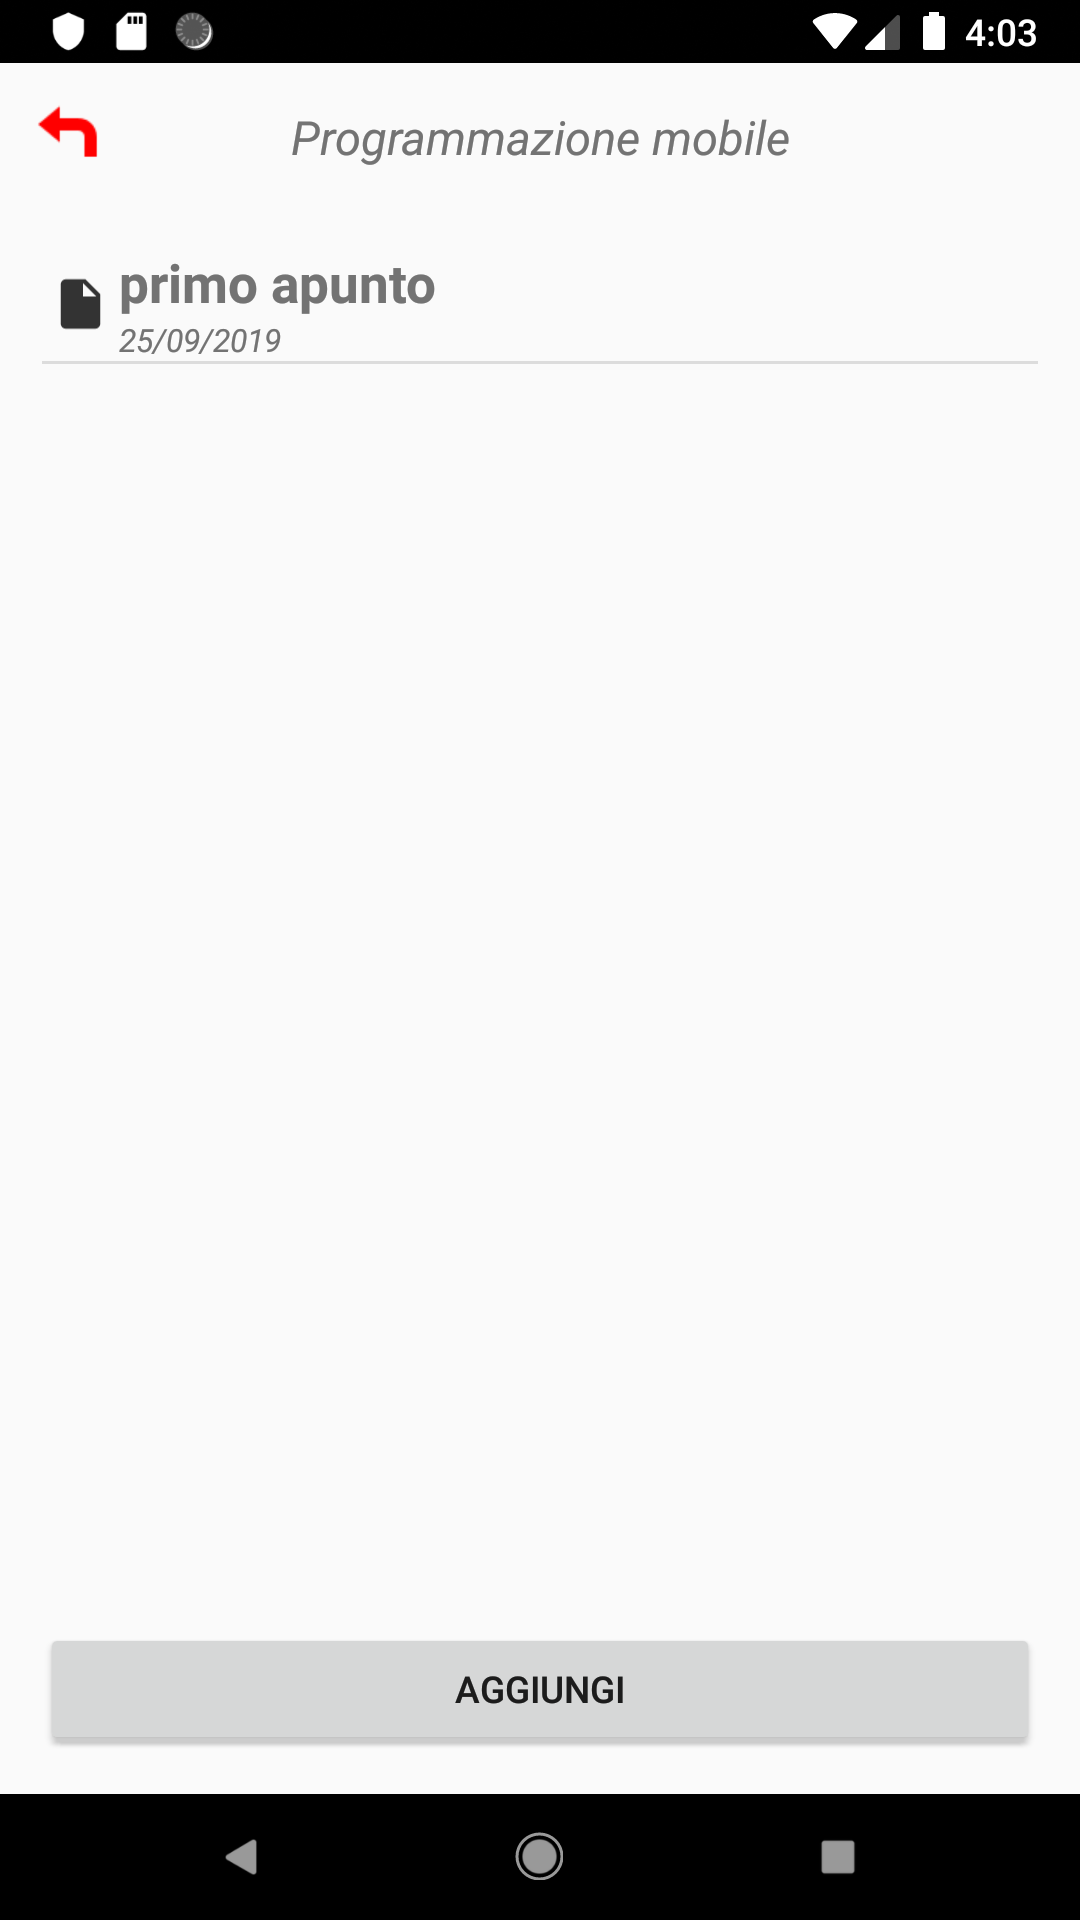
\includegraphics[width=.30\textwidth]{miei_appunti_lista_appunti}}
	\caption{\small Scegli aggiungi o elimina una materia e scegli un appunto.}
\end{figure}

Scelta la materia accediamo ad una seconda lista contenente tutti gli appunti relativi ad essa; ogni elemento della lsita contiene titolo e data relativi ad ogni appunto.
Da questa lista possiamo accedere e visualizzare l'annotazione vera e propria.

Gli appunti possono essere aggiunti con il bottone \textbf{"aggiungi"}, qui inseriremo titolo data e annotazione che vogliamo salvare; da questa schermata, inserendo la spunta nel campo \textbf{"Condividi"}, possono essere condivisi direttamente gli appunti con gli altri utenti.

Per eliminare un appunto basta tenere premuto l'elemento da eliminare, verrà attivata una finestra di dialogo da cui è possibile confermare la cancellazione.

\begin{figure}[!h]
	\centering
	{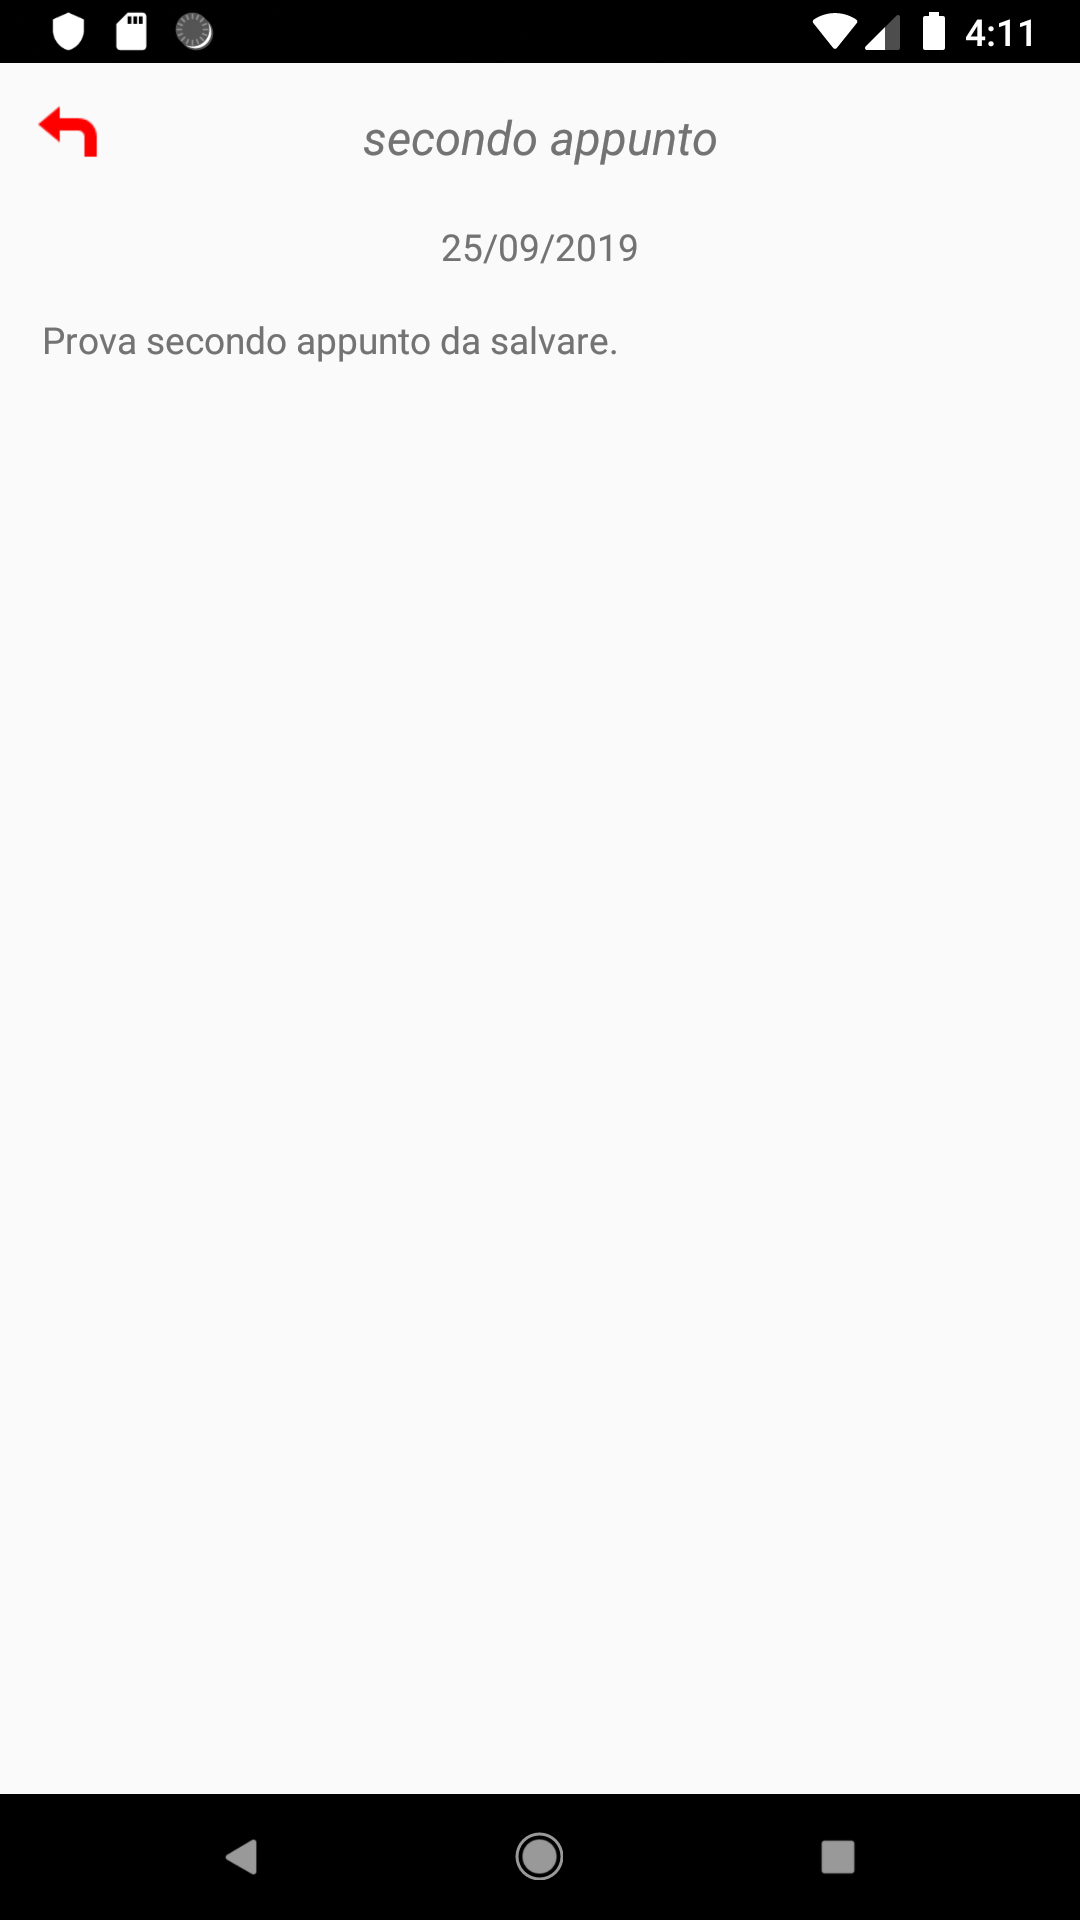
\includegraphics[width=.30\textwidth]{miei_appunti_vedi_appunto}} \quad
	{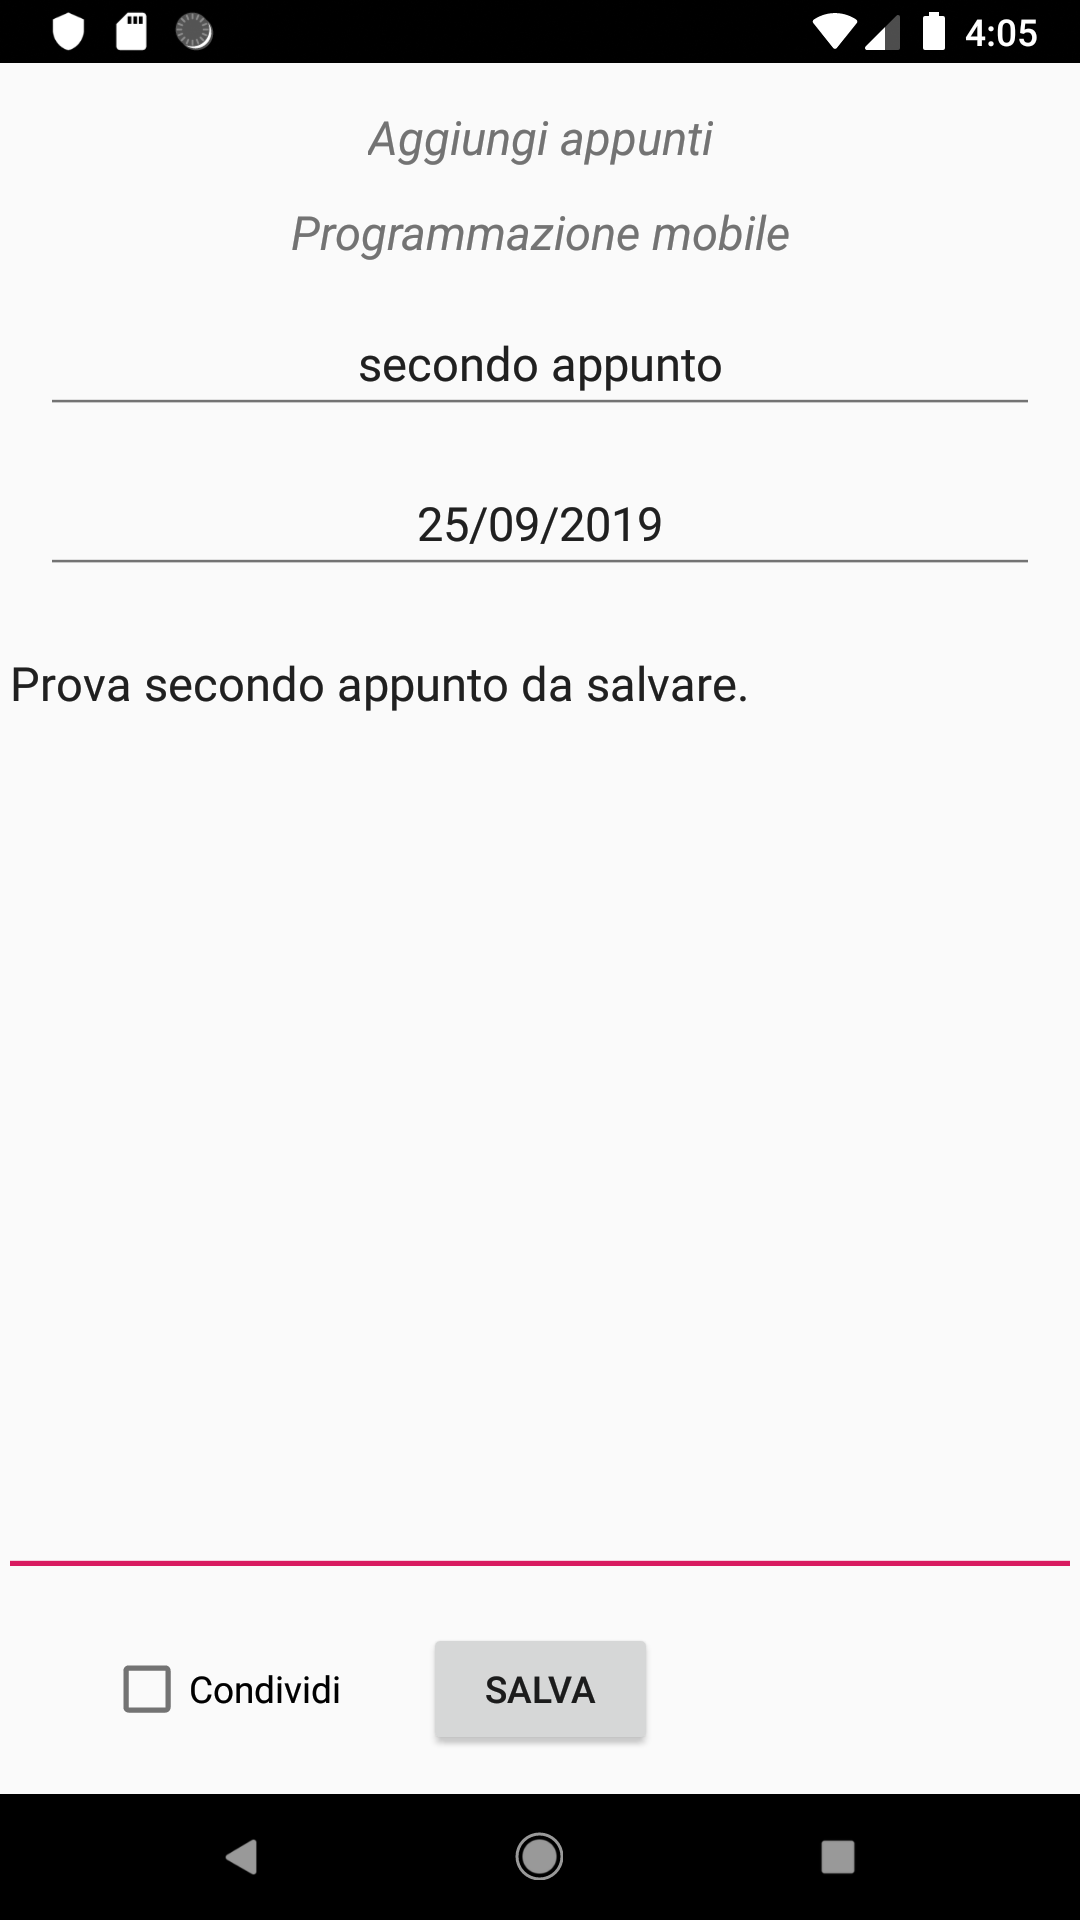
\includegraphics[width=.30\textwidth]{miei_appunti_aggiungi_appunto}} \quad
	{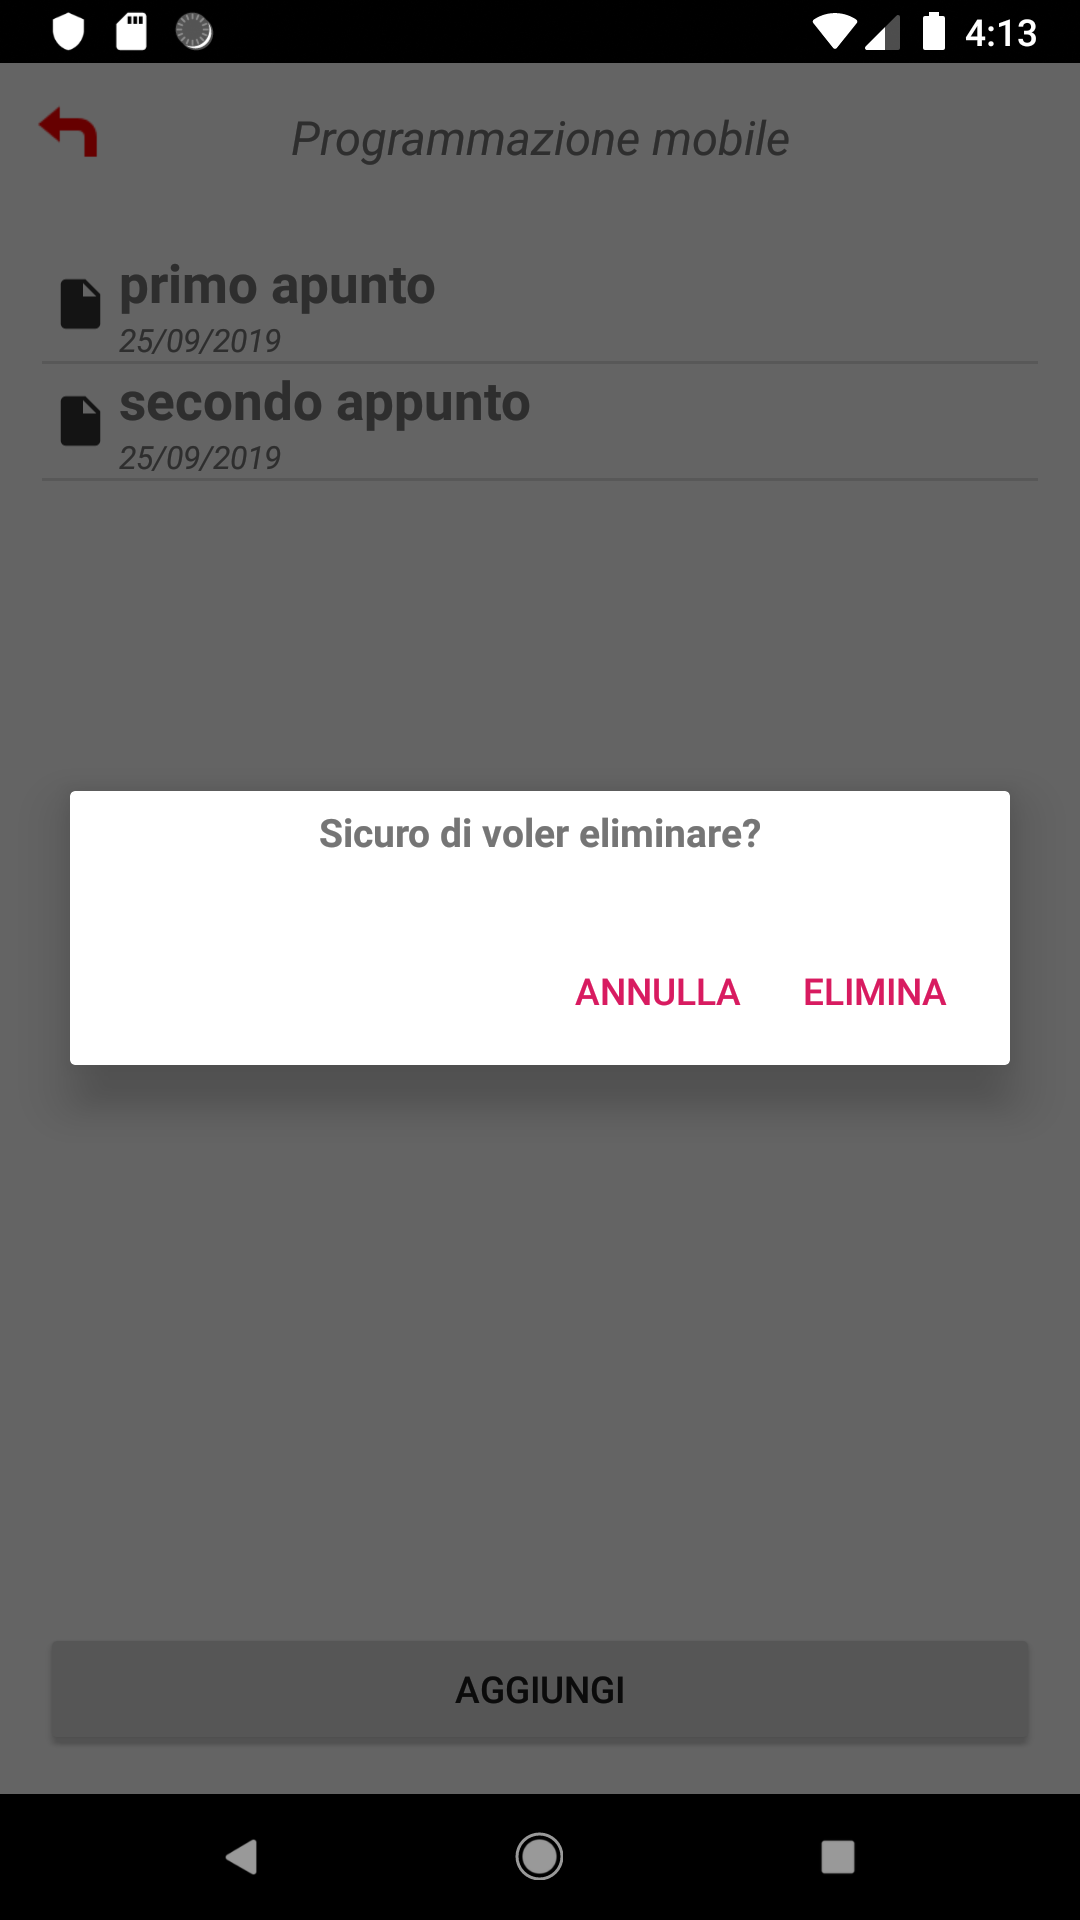
\includegraphics[width=.30\textwidth]{miei_appunti_elimina_appunto}}
	\caption{\small Visualizza, aggiungi o elimina un appunto.}
\end{figure}

\subsection{Appunti condivisi}
Nella sezione appunti condivisi possiamo scegliere una delle materie predefinite in lista per visualizzare gli appunti che sono stati condivisi ed eventualmente visualizzarli o scaricarli.

\begin{figure}[!h]
	\centering
	{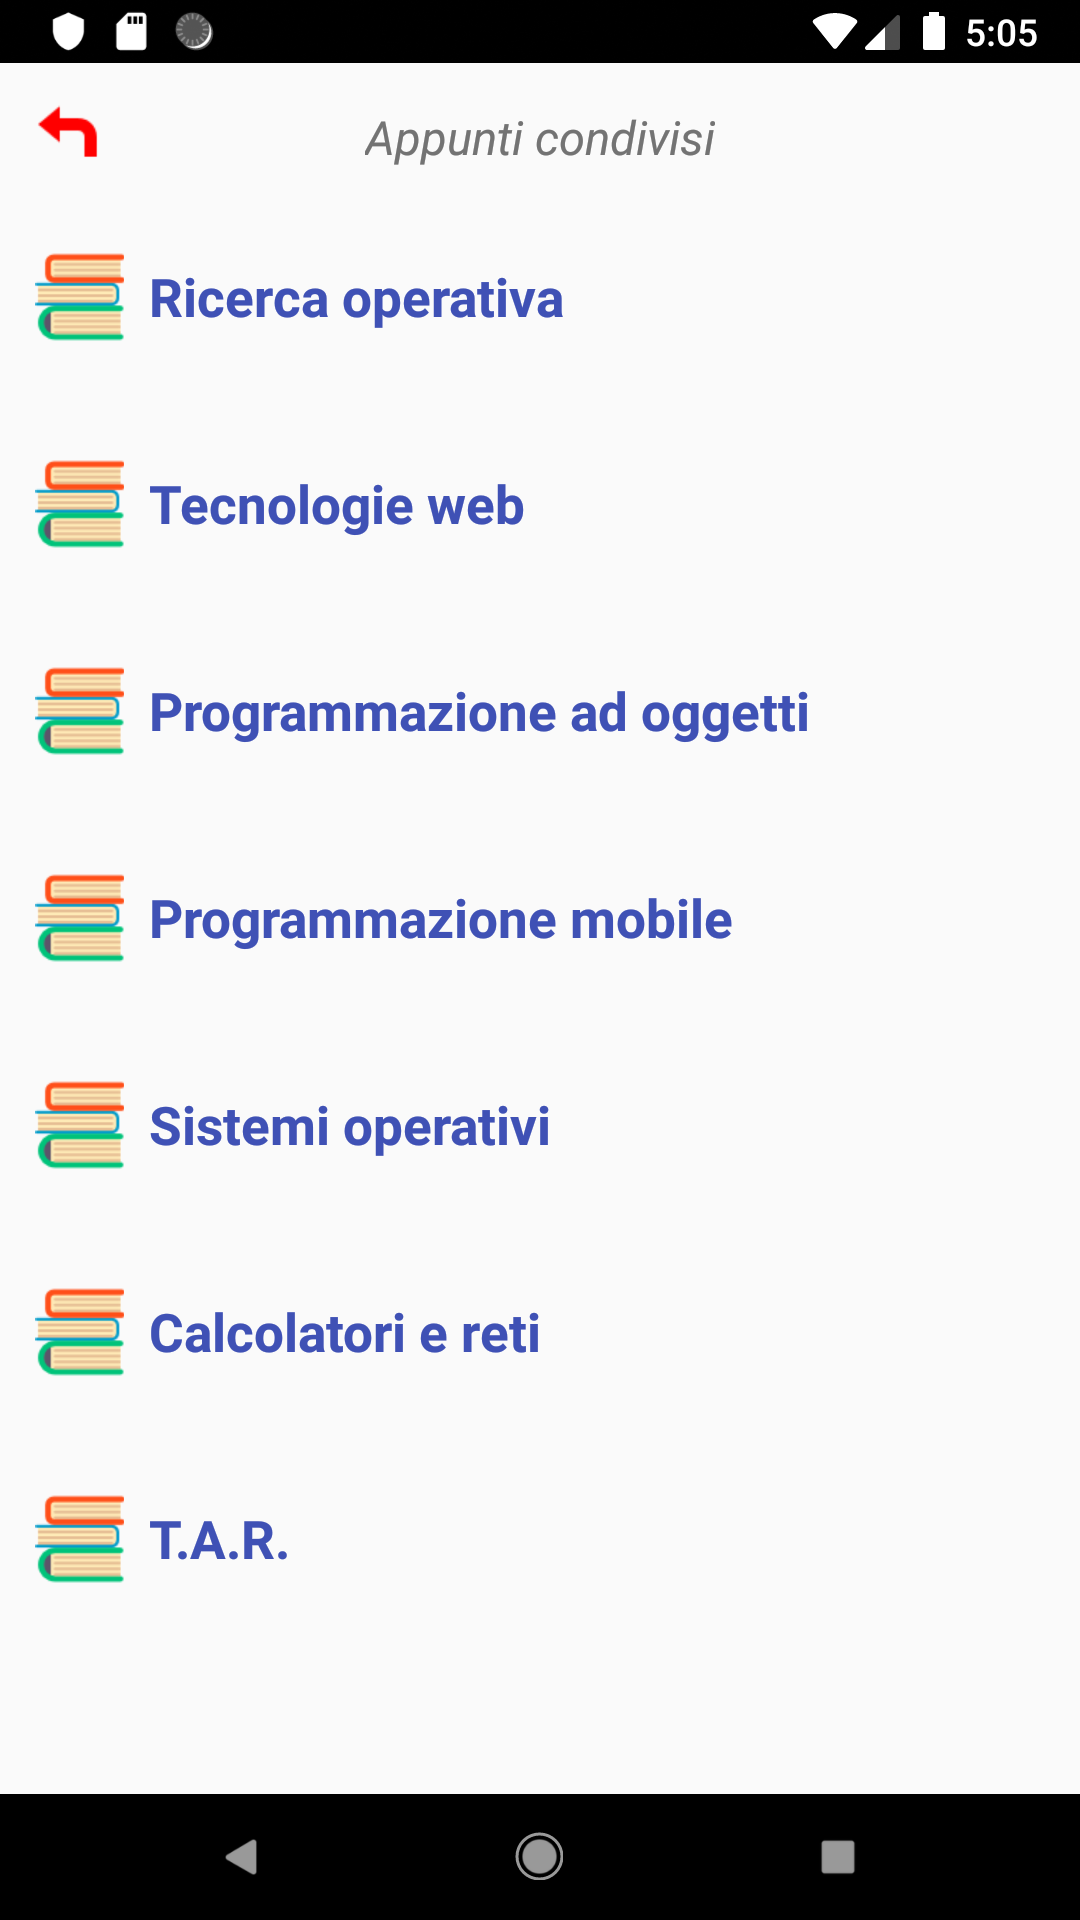
\includegraphics[width=.30\textwidth]{appunti_condivisi_lista_materie}} \quad
	{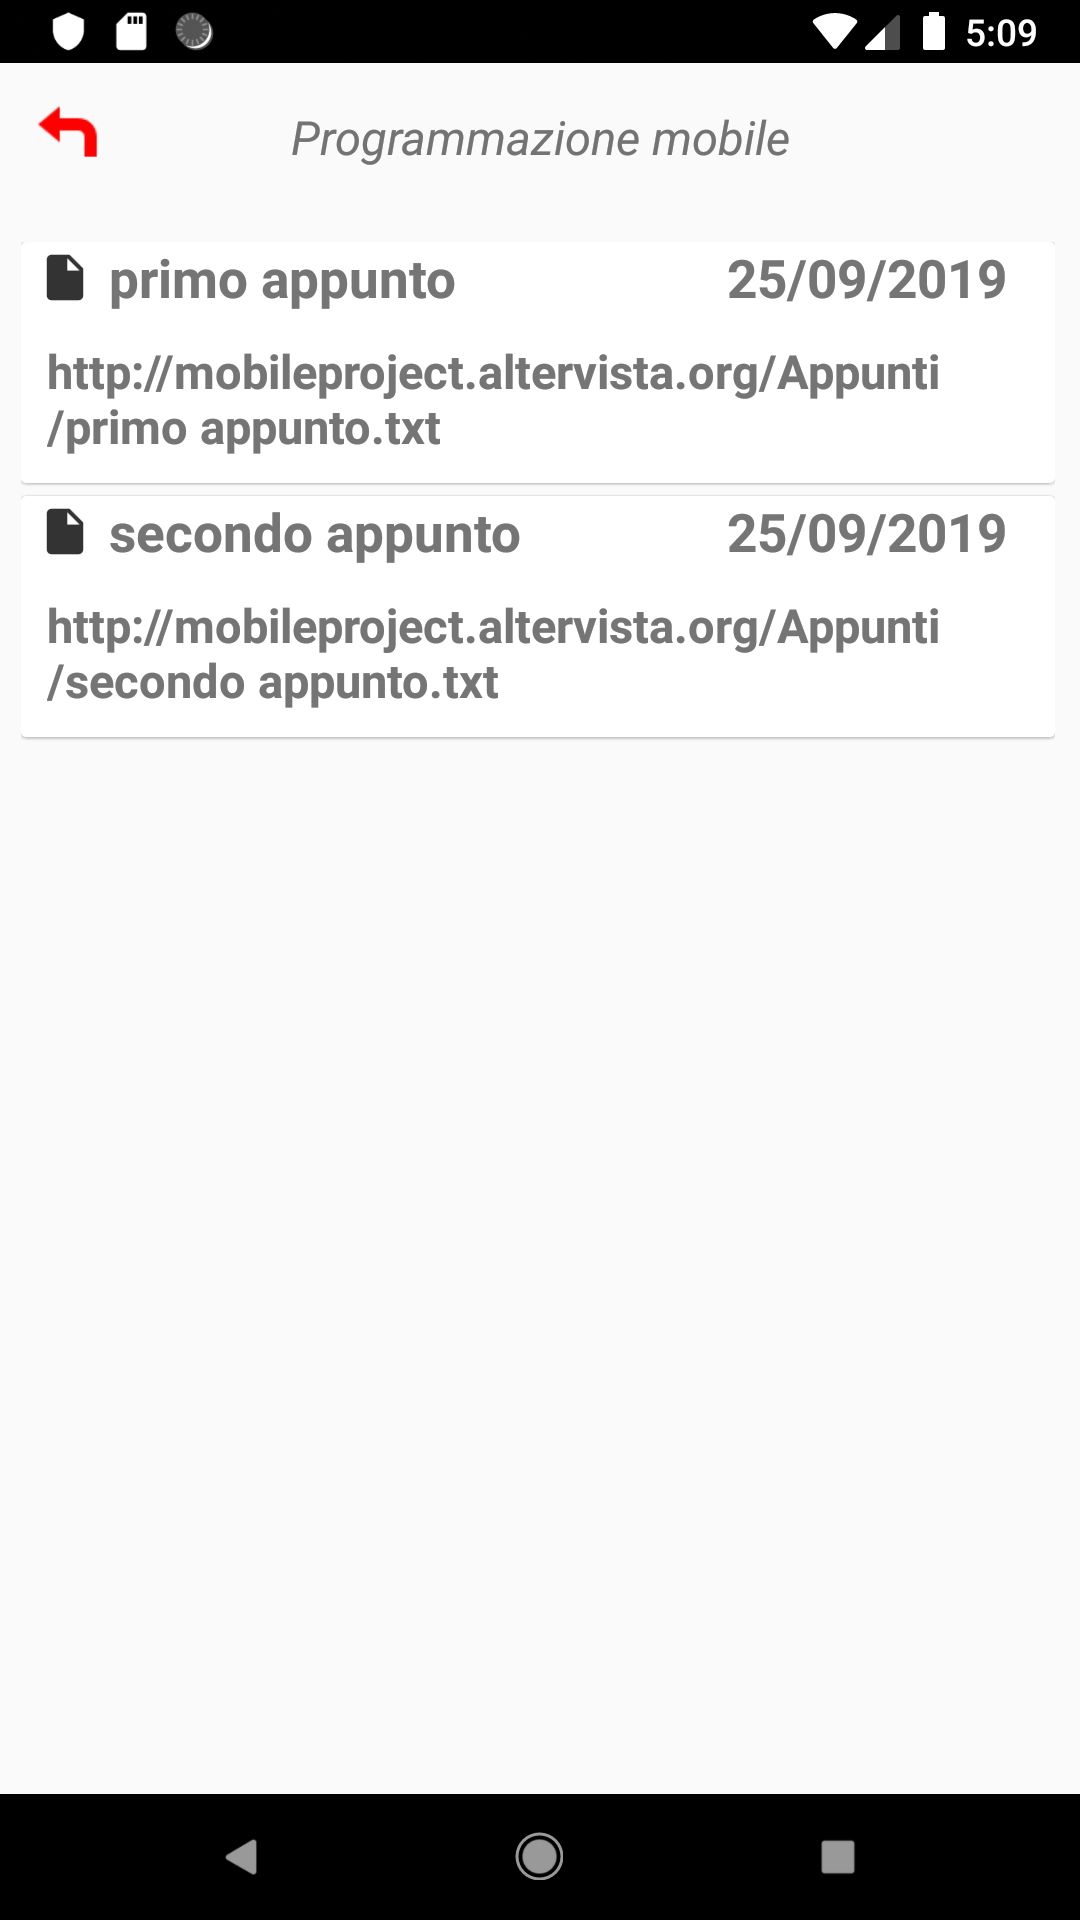
\includegraphics[width=.30\textwidth]{appunti_condivisi_lista_appunti}} \quad
	{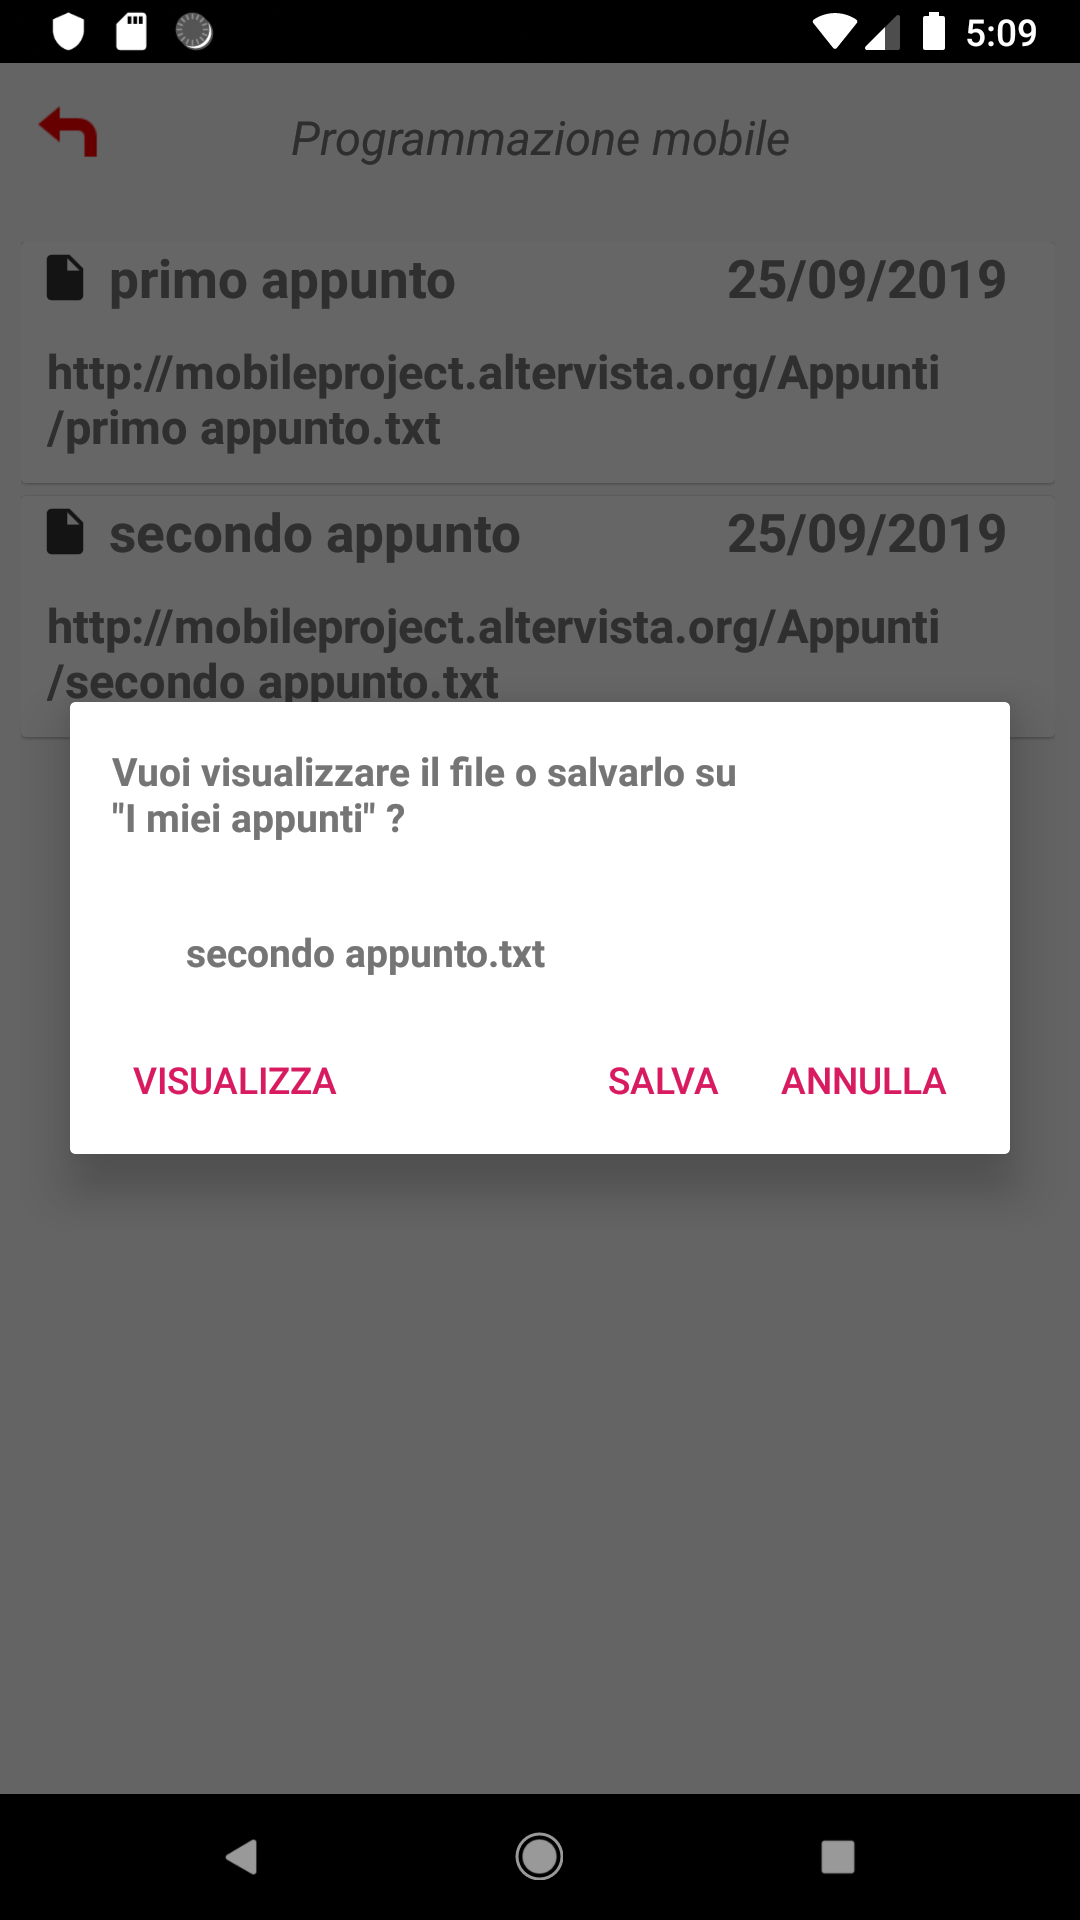
\includegraphics[width=.30\textwidth]{appunti_condivisi_scegli_azione}}
	\caption{\small Appunti condivisi, scegli la materia, scegli l'appunto, visualizza o scarica.}
\end{figure}

\subsection{Impostazioni}
Dalle impostazioni possiamo banalmente modificare \textbf{username}, \textbf{password} e leggere informazioni \textbf{about us}.

\begin{figure}[!h]
	\centering
	{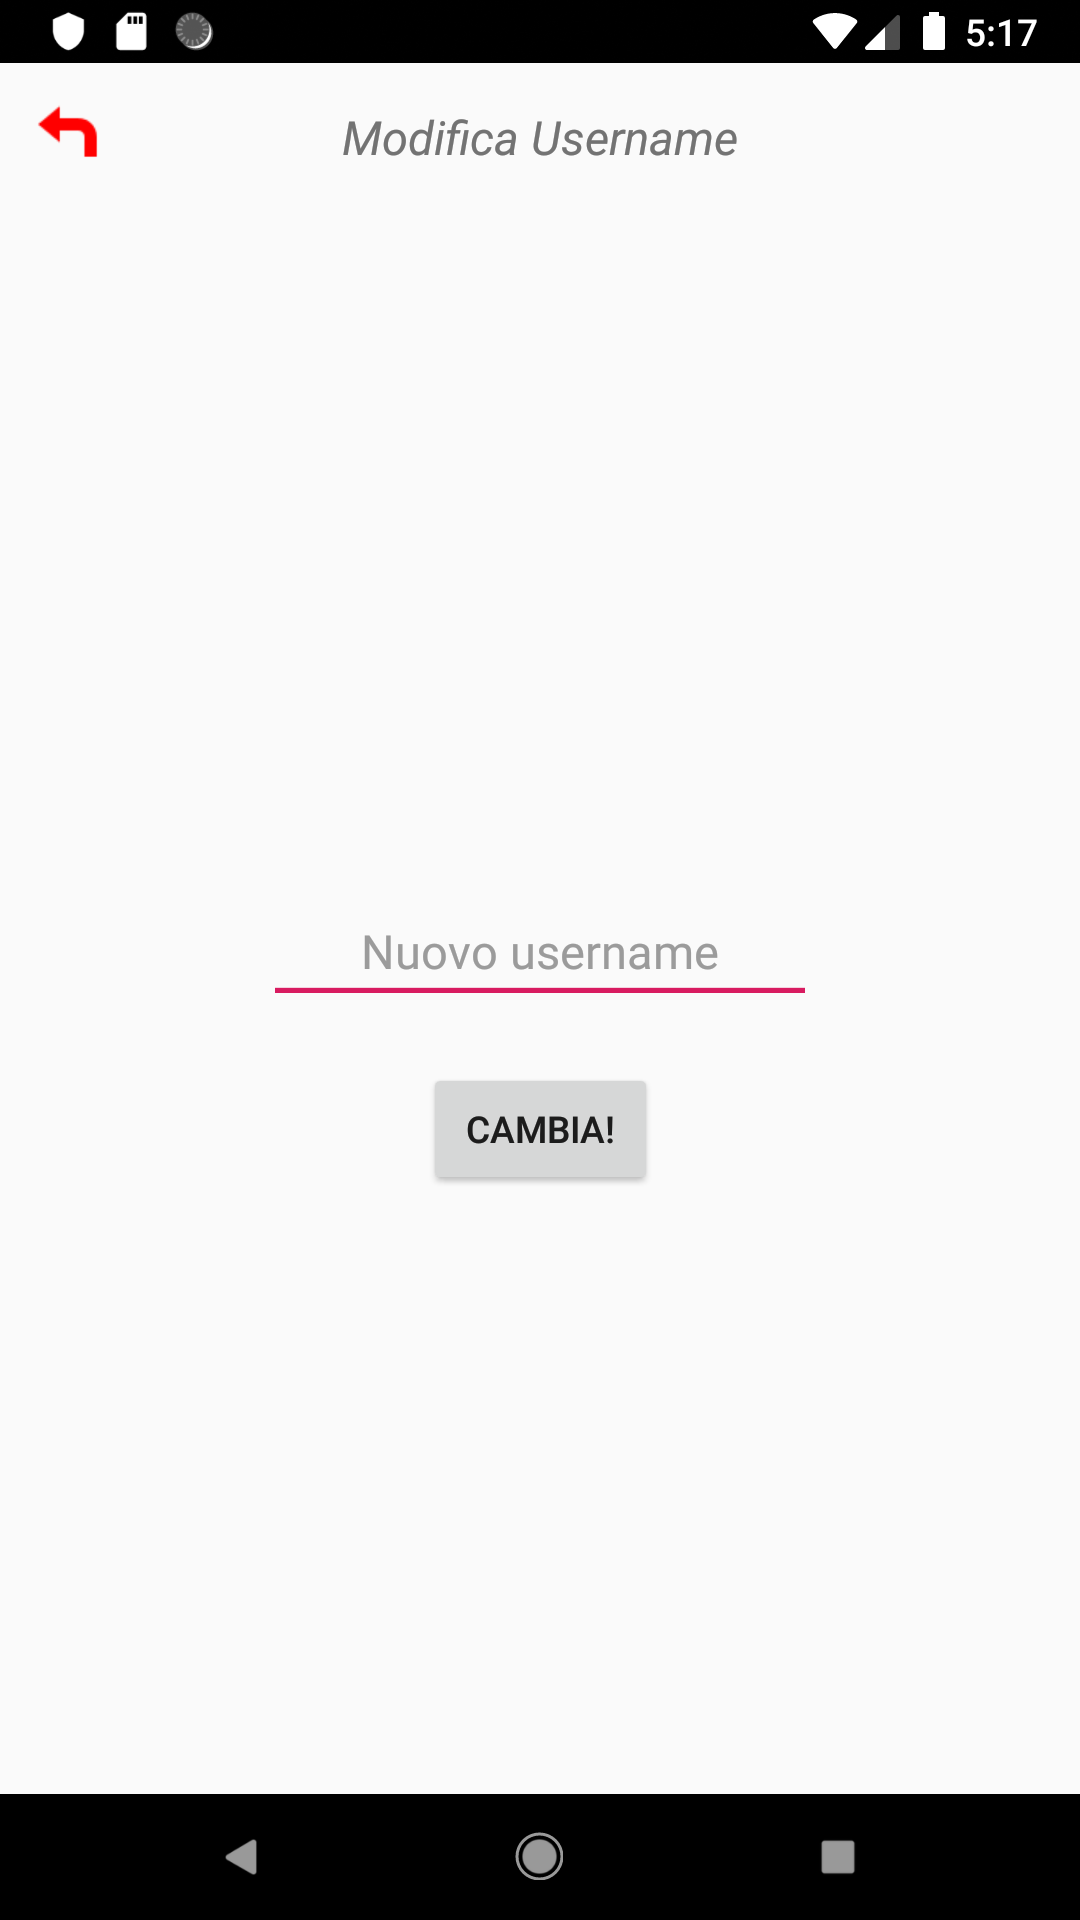
\includegraphics[width=.30\textwidth]{impostazioni_username}} \quad
	{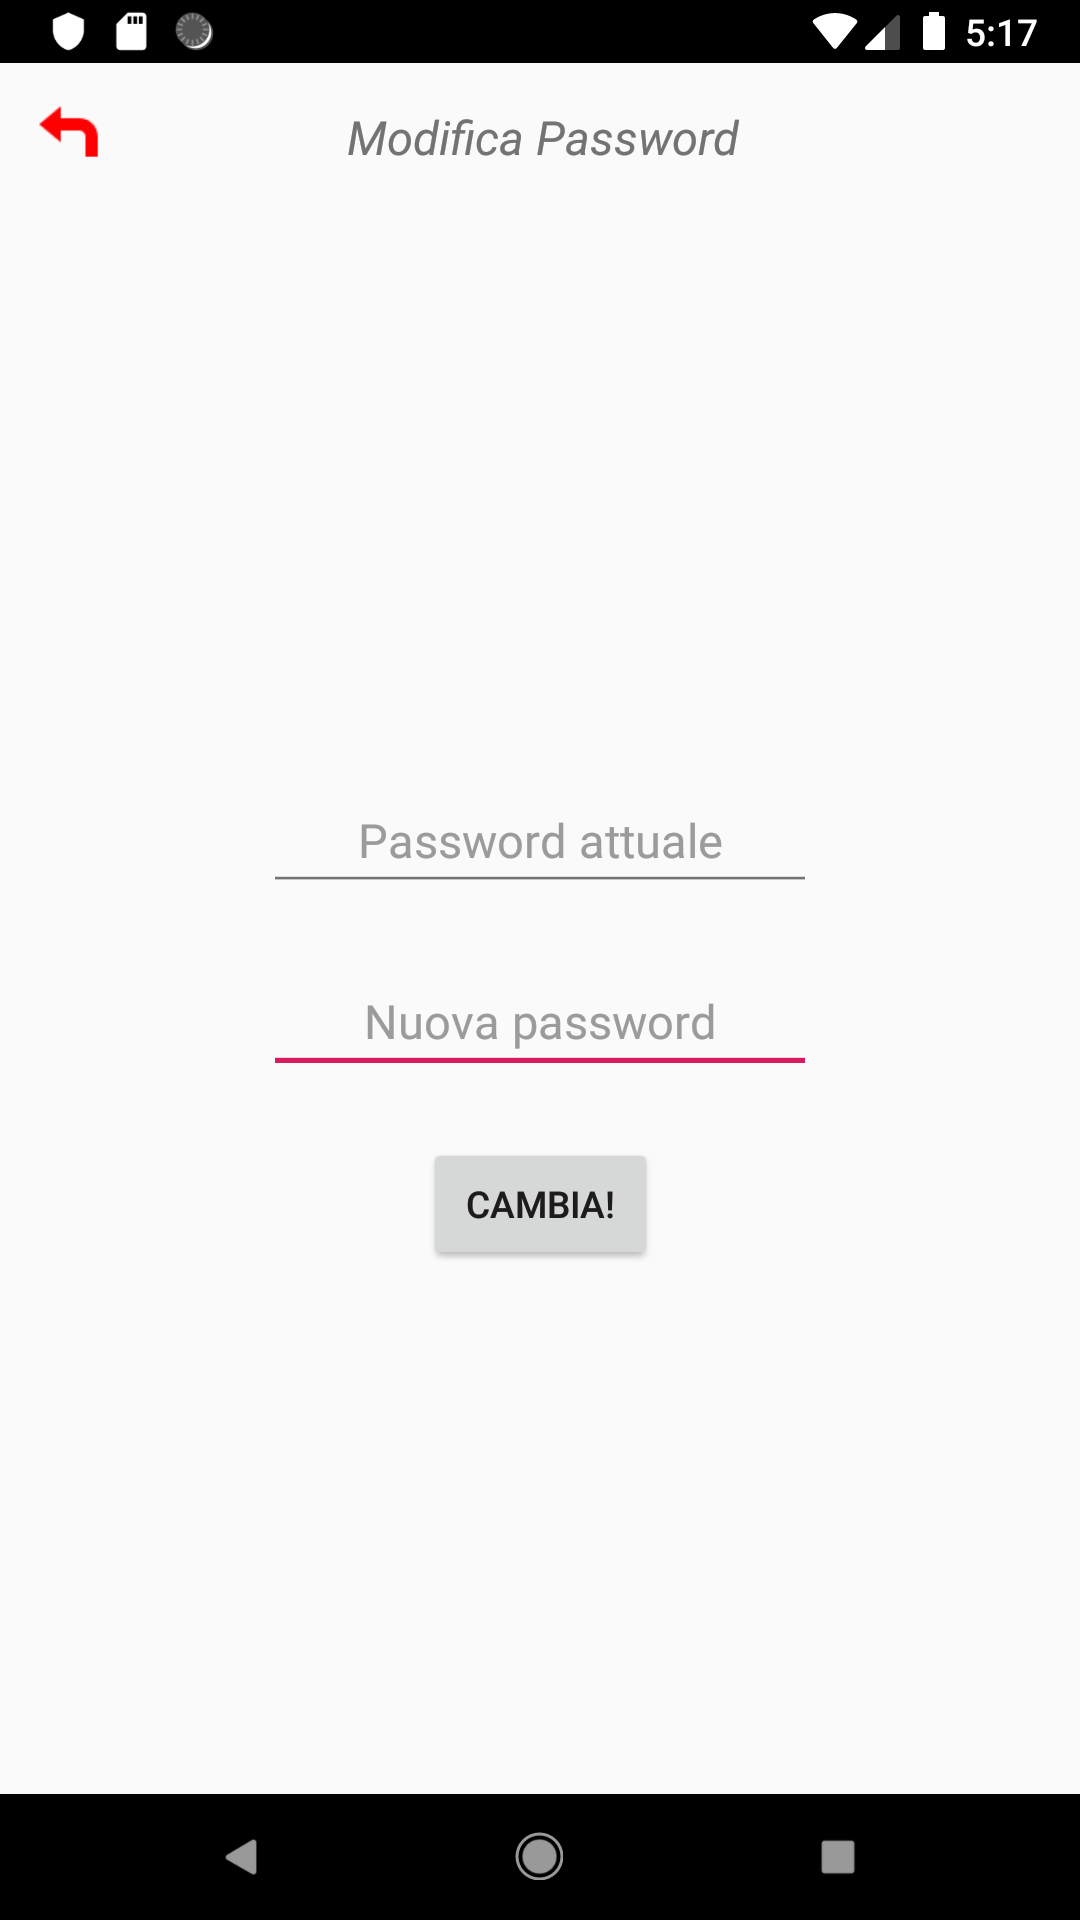
\includegraphics[width=.30\textwidth]{impostazioni_password}} \quad
	{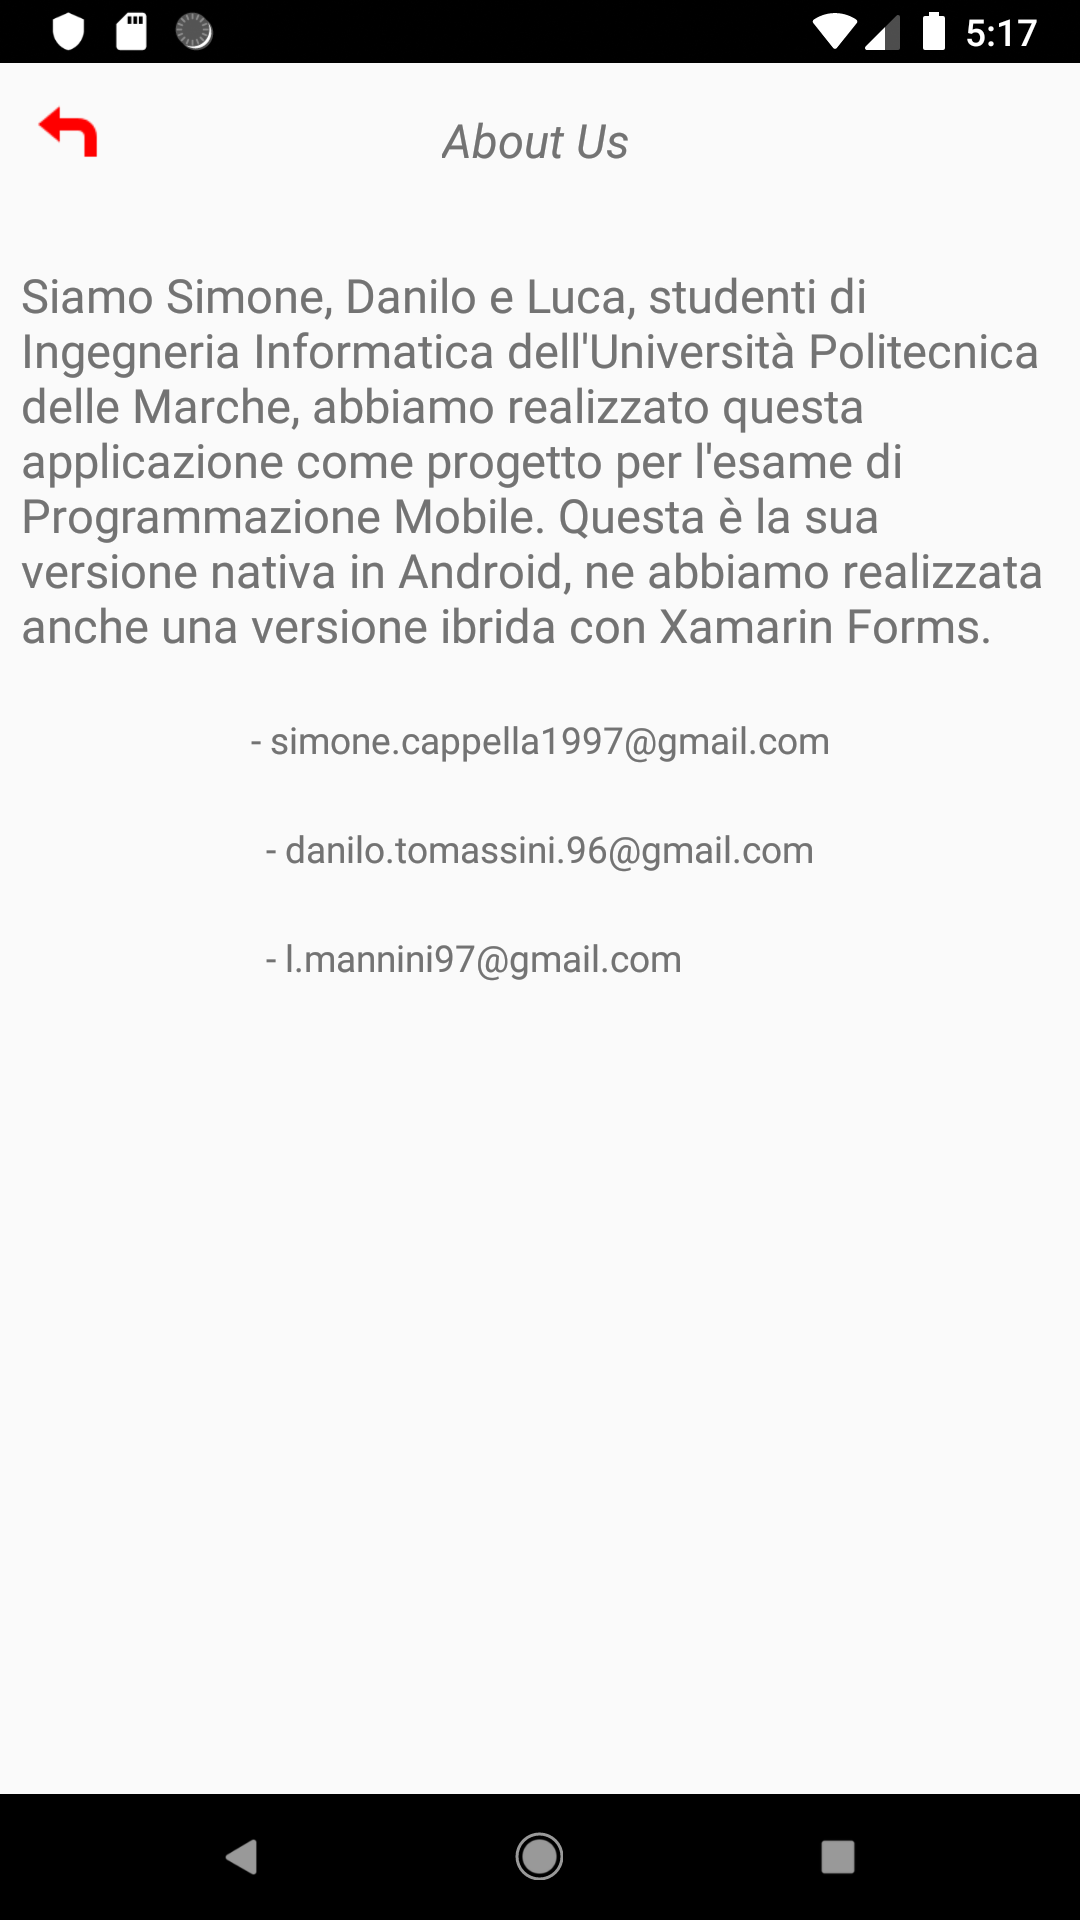
\includegraphics[width=.30\textwidth]{impostazioni_about_us}}
	\caption{\small Azioni eseguibili nelle impostazioni.}
\end{figure}
\newpage
\section{Implementazioni Android studio}
\subsection{Login e Registrazione}
Per avviare il login, ovviamente, è necessario riempire le \textbf{EditText} relative a username e password; i relativi valori verranno assegnati alle variabili \textbf{login\_name} e \textbf{login\_pass}.

La connessione al database viene instaurata indicando \textbf{method}, stringa inizializzata in precedenza a \textbf{"login"}, dati relativi ad username e password e l'url contenente il percorso fino alla funzione di login contenuta nel server.

Se la funzione del server da esito negativo non verrà effettuato il login e verrà stampato un \textbf{Toast}, per mezzo della funzione \textbf{show}. Altrimenti verrà stampato un messaggio di benvenuto e verrà lanciata la \textbf{MainActivity}.
\begin{lstlisting}
\\FirstActivity\\
[...]
public void userLogin(View view) {
[...]
try {
	Sring url = "http://mobileproject.altervista.org/login.php";
	auth = supportTask.execute(method, login_name, login_pass, url).get();
	} catch (ExecutionException e)
	{
		e.printStackTrace();
	}catch (InterruptedException a)
	{
		a.printStackTrace();
	}
	if(auth.equals("Login Success"))
	{
		launchMainActivity(view);
		show("Benvenuto "+ login_name + "!");
		finish();
	}else
	{
		show("Dati errati. Riprova.");
	}
}
[...]
\end{lstlisting}

La registrazione viene gestita in modo simile.

In un \textbf{if} viene verificato in modo veloce se le condizioni su username e password sono verificate, in caso contrario viene lanciato un avviso.

Il metodo con cui si instaura la connessione al server è lo stesso, cambiano solo gli argomenti, \textbf{url} e \textbf{method}.

Una volta che la registrazione è andata a buon fine l'attività viene interrotta e si torna alla schermata di login.

\begin{lstlisting}
\\Register\\
[...]
public void userRegister() {
[...]
if (register_name.length() >= 3 && register_pass.length() >= 3)
{
	try {
		String url = "http://mobileproject.altervista.org/register.php";
		auth= supportTask.execute(method, register_name, register_pass, url).get();
	} catch (ExecutionException e) {
		e.printStackTrace();
	} catch (InterruptedException e) {
		e.printStackTrace();
	}
	if (auth.equals("Registrazione avvenuta con successo!")) {
		show("Registrazione effettuata con successo, accedi!");
		finish();
	} else if (auth.equals("Username in uso")) {
		show("Username gia' in uso, prova con uno diverso!");
	}
}
else
{
show(I campi devono contenere almeno 3 caratteri.);
}
[...]
\end{lstlisting}

\subsection{Orario}
Avviata l'activity \textbf{orario} vengono catturate le dimensioni del display, calcolata la dimensione del \textbf{fragment} contenente la tabella dell'orario e fatto partire uno switch sul giorno corrente.

\begin{lstlisting}
\\Clock\\
[...]
protected void onCreate(Bundle savedInstanceState) {
[...]
Calendar calendar = Calendar.getInstance();
int day = calendar.get(Calendar.DAY_OF_WEEK);
Fragment fragment = null;
switch (day){
	case Calendar.MONDAY:
		fragment = new lun_fragment();
		nav.setSelectedItemId(R.id.lun);
		break;
	case Calendar.TUESDAY:
		fragment = new mar_fragment();
		nav.setSelectedItemId(R.id.mar);
		break;
	case Calendar.WEDNESDAY:
[...]
}
loadFragment(fragment);
[...]
\end{lstlisting}

Questo switch permette di caricare il fragment relativo al giorno corrente (es. se oggi è lunedì viene caricato il fragment relativo a lunedì); viene, infatti, inizializzato l'oggetto fragment e viene selezionato l'elemento sulla navbar.

\begin{lstlisting}
\\Clock\\
[...]
public boolean onNavigationItemSelected(@NonNull MenuItem item) {
Fragment fragment = null;
switch(item.getItemId())
{
	case R.id.lun:
		next = 0;
		fragment = new lun_fragment();
		break;
	case R.id.mar:
		next = 1;
		fragment = new mar_fragment();
		break;
	case R.id.mer:
		next = 2;
		fragment = new mer_fragment();
		break;
[...]
}
return loadFragment(fragment);
[...]
\end{lstlisting}

Allo stesso modo la funzione \textbf{onNavigationItemSelected}, associa in base allitem della navbar cliccato un'istanza del fragment all'oggetto fragment e nuovamente viene lanciata la funzione \textbf{loadFragment}.

La funzione \textbf{loadFragment} carica il fragment richiesto e gestisce lo scorrimento a destra o sinistra dipendentemente dalla posizione del fragment corrente rispetto a quello scelto.
\subsubsection{Fragment}
Prendiamo come riferimento il fragment relativo al \textbf{lunedì}, gli altri saranno implementati in modo analogo.

All'interno del fragment vengono nuovamente catturate le dimensioni del display e impostate le dimensioni delle varie caselle della tabella, rispettivamente:
\begin{itemize}
\item \textbf{Ora:} l'ora di inizio della lezione.
\item \textbf{Materia:} la materia inserita.
\item \textbf{Aula:} l'aula nel quale si terrà la lezione.
\item \textbf{X:} edit per cancellare la riga.
\end{itemize}

La tabella viene inizializzata nella funzione \textbf{onCreate}, qui, ogni elemento della tabella viene assegnato ad una variabile e successivamente "riempito" con il testo salvato, andadolo a recuperare con l'oggetto \textbf{sa}, della classe \textbf{SalvaOrario}, passando la chiave $\{lun\_1, lun\_2,..., lun\_11\}$ per quanto riguarda la tabella di lunedì, per la tabella di martedì le chiavi saranno costruite come $\{mar\_1,...,mar\_11\}$; la stessa logica vale per gli altri giorni; in tal modo possiamo recuperare in modo distinto le 11 materie salvate con la relativa aula per i diversi giorni.

\begin{lstlisting}
\\lun_fragment\\
[...]
public View onCreateView(LayoutInflater inflater, 
@Nullable ViewGroup container, @Nullable Bundle savedInstanceState) {
[...]
SalvaOrario sa = new SalvaOrario();
[...]
txtMat1 = v.findViewById(R.id.materia1);
txtMat1.setText(sa.getMateria("lun_1", getActivity()));
txtMat1.setOnClickListener(this);
txtAula1 = v.findViewById(R.id.aula1);
txtAula1.setText(sa.getAula("lun_1", getActivity()));
txtOra1 = v.findViewById(R.id.ora1);

txtMat2 = v.findViewById(R.id.materia2);
txtMat2.setText(sa.getMateria("lun_2", getActivity()));
txtMat2.setOnClickListener(this);
txtAula2 = v.findViewById(R.id.aula2);
txtAula2.setText(sa.getAula("lun_2", getActivity()));
txtOra2 = v.findViewById(R.id.ora2);
[...]
\end{lstlisting}

Nella funzione \textbf{onClick} viene gestita la scelta di inserire una materia nell'orario o eliminarne una dallo stesso. C'è, infatti, uno switch che gestisce il "click" nelle diverse sezioni della tabella. Abbiamo due diversi tipi di azione:
\begin{itemize}
\item \textbf{Aggiungere una materia:} per aggiungere una materia si seleziona un campo materia relativo all'ora in cui vogliamo inserirlo, questo attiverà l'elemento corrispondente nello switch che imposterà la variabile $n$, utilizzata successivamente per costruire la chiave e salvare nella classe SalvaOrario, la variabile $ora$, presa direttamente dalla view e chiama la funzione \textbf{launchList()}.
\item \textbf{Elimina una materia:} se viene selezionata la "X" sulla destra della tabella viene semplicemente "pulita" la riga corrispondente, infatti, nello switch, captato l'$edit$ corrispondente, viene impostata di nuovo la variabile $n$ per essere usata come chiave e le voci $materia$ e $aula$ vengono messe a $null$, viene lanciata, poi, la funzione \textbf{inserisciSalva()}; (la variabile $inc$ serve successivamente per inserire in un colpo solo più ore della stessa materia).
\end{itemize}
\newpage
\begin{lstlisting}
\\lun_fragment\\
[...]
public void onClick (View v) {
switch (v.getId())
{
	case R.id.materia1:
		n = 1;
		ora = txtOra1.getText().toString();
		v.startAnimation(buttonClick);
		launchList();
		break;
	case R.id.materia2:
		n = 2;
		ora = txtOra2.getText().toString();
		v.startAnimation(buttonClick);
		launchList();
		break;
[...]
	case R.id.edit1:
		n = 1;
		v.startAnimation(buttonClick);
		materia = null;
		aula = null;
		inc = 1;
		inserisciSalva();
		break;
	case R.id.edit2:
		n = 2;
		v.startAnimation(buttonClick);
		materia = null;
		aula = null;
		inc = 1;
		inserisciSalva();
		break;
[...]
\end{lstlisting}

La finzione \textbf{launchList}, chiamata nel momento in cui si vuole aggiungere una materia all'orario non fa altro che lanciare un \textbf{intent esplicito}, questo ci permette di scambiare dati tra l'activity chiamante e la chiamata, infatti tra i parametri della funzione \textbf{putExtra} abbiamo una chiave, $giorno\_ora$ e un valore, $"lunedi'" + ora$ ($ora$ è stata assegnata in precedenza nello switch). Inoltre c'è bisogno di un $REQUEST\_CODE$ utilizzato come chiave di riconoscimento tra le activity.

\begin{lstlisting}
\\lun_fragment\\
[...]
public static final int REQUEST_CODE = 0000;
[...]
public void launchList() {
	Intent intent = new Intent (getActivity(), List.class);
	intent.putExtra("giorno_ora", "lunedi'  " + ora);
	startActivityForResult(intent, REQUEST_CODE);
}
\end{lstlisting}

L'activity \textbf{List} genera la lsita predefinita delle materie da cui si può scegliere quella da inserire nella casella dell'orario scelta.

Qui i dati vengono recuperati proprio grazie alla chiave $giorno\_ora$, successivamente vengono istaziati $myDialog$ e $adapter$.

La funzione \textbf{setOnItemClickListener} chiamata per mezzo dell'oggetto $listMaterie$ e la successiva \textbf{OnItemClick} permettono di captare quale materia della lista viene scelta grazie alla sua posizione nella lista stessa.

Scelta la materia viene aperta la finestra di dialogo, all'interno di questa vengono definiti diversi elementi come una editText per l'aula e due bottoni, $- +$, questi permettono di incrementare e decrementare le ore di lezione relative alla materia.

Una volta inserita l'aula e il numero di ore si provede al salvataggio. Un listener sul bottone $btnSalva$ fa si che quando venga restituito il risultato all'activity chiamante con la variabile $intent$, questa contiene la materia scelta, l'aula e la conta delle ore, l'attivity termina con finish().
Una cosa analoga avviene nel momento in cui si decide tramite l'apposito bottone di inserire una nuova materia non contenuta nella lista predefinita.

\begin{lstlisting}
\\List\\
[...]
Intent intent = getIntent();
String giorno_ora = intent.getStringExtra("giorno_ora");
[...]
myDialog = new Dialog(this);
final ArrayAdapter<String>  adapter = new ArrayAdapter<>(this,
android.R.layout.simple_list_item_1, android.R.id.text1, listItem);
listMaterie.setAdapter(adapter);
[...]
listMaterie.setOnItemClickListener(new AdapterView.OnItemClickListener() {
	@Override
	public void onItemClick(AdapterView<?> parent, View view, int position,
	long id) {
		value = adapter.getItem(position);
[...]
myDialog.show();
[...]
btnMeno.setOnClickListener(new View.OnClickListener() {
	@Override
	public void onClick(View v) {
		i--;
		textContatore.setText(Integer.toString(i));
	}
}
[...]
btnPiu.setOnClickListener(new View.OnClickListener() {
	@Override
	public void onClick(View v) {
	i++;
	textContatore.setText(Integer.toString(i));
	}
}
[...]
btnSalva.setOnClickListener(new View.OnClickListener() {
	@Override
	public void onClick(View v) {
[...]
		Intent intent = new Intent();
		intent = intent.putExtra("mat", valore);
		setResult(Activity.RESULT_OK, intent);
		finish();
		myDialog.dismiss();
	}
[...]
\end{lstlisting}

La funzione \textbf{onActivityResult} si occupa di reperire dall'activity Lsit i risultati ottenuti dalla scelta. L'array di stringhe $res$ contiene ora nella posizione 0 la materia, nella posizione 1 l'aula e nella posizione 2 il numero di ore, che va "parsato" in un intero in quanto arrivava come una Stringa.

Viene considerato il caso in cui non si completa la scelta, in tal caso nell'activity Lista viene impostato il nome della materia a $back$ e non viene eseguita nessun'altra azione, la routine si interrompe. Nel caso in cui la scelta è stata completata i dati raccolti andranno salvati, sono passati, dunque, alla funzione \textbf{salvaOrario}.

\begin{lstlisting}
\\lun_fragment\\
[...]
public void onActivityResult(int requestCode, int resultCode, Intent data){
	super.onActivityResult(requestCode, resultCode, data);
	if ((requestCode == REQUEST_CODE) && (resultCode == Activity.RESULT_OK)) {
		String[] res = data.getStringArrayExtra("mat");
		materia = res[0];
		aula = res[1];
		inc = Integer.parseInt(res[2]);
	}
	if (materia.equals("back")){}
	else{
		salvaOrario(i, materia, aula);
	}
}
[...]
\end{lstlisting}

La funzione \textbf{salvaOrario} va a definire un cursore che sarà popolato con l'elemento del database trovato dal metodo \textbf{searchM} (questo trova nel database l'elemento il cui campo materia ha lo stesso nome della materia inserita).
Questo cursore permette di verificare, grazie all'$if$ se la materia inserita è gia presente nel database contenente le materie, in caso positivo il vecchio elemento viene eliminato; successivamente si inserisce nel database delle materie il nuovo elemento e viene chiamata la funzione \textbf{inserisciSalva()}.

Le materie vengono inserite nel database delle materie per permettere alla sezione $miei appunti$ di rendere disponibili le materie inserite nell'orario.

\begin{lstlisting}
\\lun_fragment\\
[...]
public void salvaOrario (String key, String materia, String aula) {
	Cursor c;
	c = dm.searchM(materia);
	if (c.getCount() > 0) {
		dm.delete(materia);
	}
	dm.insert(materia, ora, aula, key);
	inserisciSalva();
[...]
\end{lstlisting}

La funzione \textbf{inserisciSalva} permette di salvare, nuovamente tramite i metodi della classe \textbf{Salva Orario}, materia e aula scelti e nuovamente di aggiornare i valori delle $txtMat$ e $txtAula$.

Il \textbf{while} all'interno della funzione ripete il ciclo finchè la variabile $inc$ che conteneva la conta delle ore non arriva a 0; la Stringa $q$ viene costruita in modo da diventare una chiave per i metodi della classe SalvaOrario, infatti la variabile $i$ contiele la stringa "lun\_" e la variabile $n$ contiene il numero dipendentemente dalla riga scelta dalla tabella. Le variabili $n$ ed $inc$ alla fine del ciclo vengono rispettivamente incrementata e decrementata, questo permette di salvare in un solo colpo stessa materia e stessa aula all'interno della tabella, infatti il numero dell'elemento della tabella incrementa finche non si esaurisce il numero di ore deciso nella finestra di dialogo nell'activity List.

Lo \textbf{switch} su $n$ ha il compito di aggiornare immediatamente il valore della tabella nella posizione $n$.
\begin{lstlisting}
\\lun_fragment\\
[...]
public void inserisciSalva(){
	while (inc > 0){
		String q = i + n;
		sa.setMateria(q, materia, getActivity());
		sa.setAula(q, aula, getActivity());
		switch (n){
			case 1:
				txtMat1.setText(sa.getMateria(q, getActivity()));
				txtAula1.setText(sa.getAula(q, getActivity()));
				break;
			case 2:
				txtMat2.setText(sa.getMateria(q, getActivity()));
				txtAula2.setText(sa.getAula(q, getActivity()));
				break;
[...]
	}
	n++;
	inc--;
}
[...]
\end{lstlisting}

La classe \textbf{SalvaOrario} gestisce salvataggio ed estrazione per mezzo delle \textbf{SharedPreferences} di materia e aula.

Al suo interno sono presenti, infatti, quattro metodi:
\begin{itemize}
\item \textbf{setMateria:} prende tra gli argomenti chiave e materia e va a salvare la materia con tale chiave.
\item \textbf{getMateria:} va ad estrarre dai salvataggi la materia corrispondente alla chiave di ricerca.
\item \textbf{setAula:} di nuovo prende tra gli argomenti chiave ed aula (in questo caso la chiave viene combinata con la stringa $"\_A"$ per caratterizzare le chiavi relative alle aule) salva, dunque, il nome dell'aula.
\item \textbf{getAula:} estrae l'aula dai salvataggi per mezzo della chiave combinata con la stringa di cui sopra.
\end{itemize}

\begin{lstlisting}
\\SalvaOrario\\
[...]
public static void setMateria(String key, String value,  Context context) {
	SharedPreferences.Editor editor = preferences.edit();
	editor.putString(key, value);
	editor.commit();
}
public static String getMateria(String key, Context context)
{
	return preferences.getString(key, null);
}
public static void setAula(String key, String value,  Context context) {
	SharedPreferences.Editor editor = preferences.edit();
	editor.putString(key+"_A", value);
	editor.commit();
}
public static String getAula(String key, Context context) {
	return preferences.getString(key+ "_A", null);
}
\end{lstlisting}

\newpage
\subsection{I miei appunti}
Avviata l'activity \textbf{i miei appunti} viene mostrata la lista delle materie salvate nell'applicazione, queste sono il risultato delle materie aggiunte nell'orario o eventualmente aggiunte nella sezione in questione.

All'avvio si definisce e istanzia un cursore che va ad estrarre tutti gli elementi dal database e con un $CursorAdapter$ va a popolare la lsita. Nuovamente viene utilizzato un $onItemClickListener$ che permette di catturare l'elemento dalla lista, viene, dunque, chiamata l'activity \textbf{Notes\_Page} con un intent passando il parametro $a$, stringa che contiene il nome della materia scelta.

\begin{lstlisting}
\\MyNotes\\
[...]
protected void onCreate(Bundle savedInstanceState) {
[...]
cursor = dm.selectAll();
[...]
adapter = new SimpleCursorAdapter(this, R.layout.list_mat, cursor, 
	fromColumns, viewsList, 0);
listMat.setAdapter(adapter);
listMat.setOnItemClickListener(new AdapterView.OnItemClickListener() {
	@Override
	public void onItemClick(AdapterView<?> parent, View view, 
		int position, long id) {
		Cursor c = adapter.getCursor();
		String a = c.getString(2);
		Intent i = new Intent(getApplication(), Notes_Page.class);
		i.putExtra("mat", a);
		startActivity(i);
	}
}
[...]
\end{lstlisting}

\subsubsection{Aggiungi una materia}
Possiamo aggiungere manualmente una nuova materia o, eventualmente, eliminarne una contenuta nel database attivando il relativo bottone. Viene lanciata con un intent esplicito l'activity \textbf{AggMaterie}; si utilizza un intent esplicito per permettere l'aggiornamento della lista una volta aggiunta o eliminata una materia dalla stessa. Nella funzione \textbf{onActivityResult}, infatti, appurata la validità del ritorno dall'activity si estrae il dato, $res$ contiene il nome della materia aggiunta, e definito un nuovo cursore $nc$ si applicano metodi quali \textbf{changeCursor} sull'adapter in modo da indicargli il nuovo cursore da utilizzare e la \textbf{notifyDataSetChanged}; in tal modo la lista verrà aggiornata.

\begin{lstlisting}
\\MyNotes\\
[...]
public static final int REQUEST_CODE2 = 2222;
[...]
private void launchAggMat() {
	Intent intent = new Intent(this, AggMaterie.class);
	intent.putExtra("app", "agg materie");
	startActivityForResult(intent, REQUEST_CODE2);
}
@Override
public void onActivityResult(int requestCode, int resultCode, Intent data){
	super.onActivityResult(requestCode, resultCode, data);
	if ((requestCode == REQUEST_CODE2) && (resultCode == Activity.RESULT_OK)) {
		String res = data.getStringExtra("res");
		Toast.makeText(getApplicationContext(), res, Toast.LENGTH_SHORT).show();
	}
	Cursor nc;
	nc = dm.selectAll();
	adapter.changeCursor(nc);
	adapter.notifyDataSetChanged();
}
[...]
\end{lstlisting}

L'activity \textbf{AggMaterie} consiste di una $editText$ e due bottoni, uno per salvare la materia inserita nella edit e una per eliminarla.
Nella funzione \textbf{onCreate} dell'activity AggMaterie viene "raccolto" l'intent.

Le funzioni relative al salvataggio ed eliminazione sono implementate direttamente nella funzione \textbf{onClick}, con uno switch sull'elemento della vista cliccato.
\begin{itemize}
\item \textbf{Salva:} viene estratta la stringa e istanziato un cursore; tramite il cursore si va a cercare nel database un elemento il cui campo materia sia uguale alla materia inserita, nell'\textbf{if} viene dunque controllato tramite il metodo \textbf{getCount} sul cursore se tale elemento è stato trovato o meno, in caso positivo viene solo lanciato un avviso, altrimenti può essere salvata la nuova materia e terminata l'activity impostando il risultato dell'intent.
\item \textbf{Elimina:} si estrae nuovamente la stringa dalla edit, si istanzia il cursore e nuovamente si procede alla ricerca di un elemento il cui campo materia corrisponda alla materia scelta, stavolta nel caso in cui venga trovata viene eliminata e terminata l'activity.
\end{itemize}

\begin{lstlisting}
\\AggMaterie\\
[...]
protected void onCreate(Bundle savedInstanceState) {
[...]
	Intent intent = getIntent();
}
[...]
@Override
public void onClick(View v) {
	switch (v.getId()){
[...]
		case R.id.btnInsert:
			materia = editMateria.getText().toString();
			Cursor c = dm.searchM(materia);
			if(c.getCount() > 0){
				[...]
			}else{
				dm.insert(materia, "ora", "aula", "code");
				Intent res  = new Intent();
				res = res.putExtra("res", materia);
				setResult(Activity.RESULT_OK, res);	
				finish();
			}
			break;
		case R.id.btnDelete:
			String materia = editMateria.getText().toString();
			Cursor del = dm.searchM(materia);
			if (del.getCount() > 0){
				dm.delete(materia);
				finish();
			}
			[...]
			break;
	}
}
[...]
\end{lstlisting}

\subsubsection{Vedi appunti}
Scelta la materia dalla lista visualizzata all'avvio di \textbf{MyNotes} viene lanciata, come visto, l'activity \textbf{Notes\_Page}.

All'avvio viene subito estratto il dato passato dall'activity chiamante, si tratta del nome della materia scelta, successivamente vengono definiti un \textbf{cursore} che contiene gli elementi del database la cui materia coincide con quella ricevuta in $a$ e un \textbf{adapter} che permette di riempire la lista con gli elementi del cursore, in particolare vengono messi nella lista titolo e data dell'appunto.

\begin{lstlisting}
\\Notes_Page\\
[...]
protected void onCreate(Bundle savedInstanceState) {
	[...]
	Intent r = getIntent();
	a = r.getStringExtra("mat");
	[...]
	cursor = da.searchM(a);
	adapter = new SimpleCursorAdapter(this, R.layout.list_app_loc, cursor,
		fromColumns, viewsList, 0);
	listNote.setAdapter(adapter);
	[...]
\end{lstlisting}

In tal caso abbiamo due possibili eventi sulla lista, un click singolo o un click prolungato (longClick).
\begin{itemize}
\item \textbf{Click:} la funzione \textbf{onItemClick} gestisce il click singolo sull'elemento, grazie alla posizione viene istanziato un nuovo cursore all'elemento in questione e ne vengono estratti come stringhe $materia, titolo, data e l'appunto vero e proprio$, viene, dunque, stampato a schermo un \textbf{Toast} contenente il titolo dell'appunto scelto e viene lanciata la funzione \textbf{launchVedi}.
\item \textbf{LongClick:} il long click permette di eliminare l'appunto. Viene nuovamente istanziato un cursore attraverso il quale vado ad estrarre $code$ e $titolo$ dell'appunto selezionato.

Viene successivamente costruita una finestra di dialogo grazie alla classe AlertDialog. Nell'alert dialog devono essere settati i bottoni "positivo" e "negativo", rispettivamente grazie a \textbf{setPositiveButton} e \textbf{setNegativeButton}.

Settato il positive button al suo interno viene utilizzata una funzione \textbf{onClick} che al click fa partire il metodo \textbf{delete} della classe \textbf{DataAppLoc}, database per gli appunti, che va a cancellare l'appunto andandolo a cercare con la variabile $code$. Successivamente viene aggiornata la lista come nelle activity precedenti e costruita la stringa con il percorso del file questo viene cancellato.

Il set del negative button non implementa nessuna funzione, in tal caso la alert dialog viene chiusa.
\end{itemize}

\begin{lstlisting}
\\Notes_Page\\
[...]
da = new DataAppLoc(this);
[...]
listNote.setOnItemClickListener(new AdapterView.OnItemClickListener() {
	@Override
	public void onItemClick(AdapterView<?> parent, View view, int position,
		long id) {
		Cursor c = adapter.getCursor();
		code = c.getString(0);
		String materia = c.getString(1);
		String titolo = c.getString(3);
		String data = c.getString(2);
		String app = c.getString(4);
		Toast.makeText(getApplicationContext(), code, Toast.LENGTH_SHORT).show();
		launchVedi(materia, titolo, data, app);
	}
	@Override
	public boolean onItemLongClick(AdapterView<?> parent, final View view,
		final int position, long id) {
		Cursor c = adapter.getCursor();
		code = c.getString(0);
		final String titolo = c.getString(3);
		[...]
		LayoutInflater inflater = LayoutInflater.from(context);
		View mess = inflater.inflate(R.layout.messaggio_elimina,null);
		AlertDialog.Builder alertDialogBuilder = new AlertDialog.Builder(context);
		alertDialogBuilder.setView(mess);
		alertDialogBuilder.setPositiveButton("ELIMINA",
			new DialogInterface.OnClickListener() {
			@Override
			public void onClick(DialogInterface dialog, int which) {
				da.delete (code);
				Cursor nc;
				nc = da.searchM(a);
				adapter.changeCursor(nc);
				adapter.notifyDataSetChanged();
				Context context = getApplicationContext();
				String folder = context.getFilesDir().getAbsolutePath()
					+ File.separator + "Appunti/";
				File file = new File(folder + titolo + ".txt");
				boolean deleted = file.delete();
			}
		}
		alertDialogBuilder.setNegativeButton("ANNULLA",
			new DialogInterface.OnClickListener() {
			@Override
			public void onClick(DialogInterface dialog, int which) {}
		}
		[...]
\end{lstlisting}

Come già detto nel caso di un singolo click su un elemento della lista viene chiamata la funzione \textbf{launchVedi}, questa crea un intent e un bundle contenente nome della materia cui si riferisce, titolo dell'appunto, data e annotazioni, questo bundle viene inserito nell'intent con il quale sarà chiamata l'activity \textbf{VediAppunti}.

\begin{lstlisting}
\\Notes_Page\\
[...]
public void launchVedi(String materia, String titolo, String data, String app){
	Intent i = new Intent(getApplication(), VediAppunti.class);
	Bundle bundle = new Bundle();
	bundle.putString("materia", materia);
	bundle.putString("titolo", titolo);
	bundle.putString("data", data);
	bundle.putString("app", app);
	i.putExtra("data", bundle);
	startActivity(i);
}
\end{lstlisting}

Nel caso in cui si voglia aggiungere un appunto va attivato il bottone \textbf{Aggiungi}, il cui evento è catturato nella funzione \textbf{onClick} della classe; questa banalmente chiama la funzione \textbf{launchAggiungi}.

La funzione in questione si occupa semplicemente di utilizzare un intent esplicito che va a lanciare l'activity \textbf{AggiungiAppuntiLoc}

\begin{lstlisting}
\\Notes_Page\\
[...]
public void launchAggiungi(){
	Intent intent = new Intent(this, AggiungiAppuntiLoc.class);
	intent.putExtra("app", a);
	startActivityForResult(intent, REQUEST_CODE1);
}
[...]
\end{lstlisting}

L'activity \textbf{AggiungiAppuntiLoc} si occupa di salvare gli appunti in locale ed eventualmente nella sezione per gli appunti condivisi.

Per quanto riguarda il salvataggio in locale, nella funzione \textbf{onClick} della classe nel caso in cui venga attivato il bottone $salva$ vengono salvati i testi inseriti delle edit e i dati vengono salvati nel database relativo agli appunti, viene, quindi, restituito l'intent con la variabile $res$ con una semplice stringa $"Appunti salvati"$.

\begin{lstlisting}
\\AggiungiAppuntiLoc\\
[...]
public void onClick(View v) {
[...]
	case R.id.btnSalvaApp:
		final String titolo = editTitolo.getText().toString();
		String data = editData.getText().toString();
		String appunti = editApp.getText().toString();
		da.insert(a, data, titolo, appunti);
		String res = "Appunti salvati";
		Intent intent = new Intent();
		intent = intent.putExtra("res", res);
		setResult(Activity.RESULT_OK, intent);
[...]
\end{lstlisting}

Terminata l'activity per salvare nuovi appunti si torna alla Notes\_Page, qui la funzione \textbf{onActivityResult} come al solito controlla il risultato dell'activity chiamata con il $REQUEST\_CODE$ e il $RESULT\_OK$, verificata la validità viene stampato il messaggio per la conferma del salvataggio e successivamente aggiornata la view della lista.

\begin{lstlisting}
public void onActivityResult(int requestCode, int resultCode, Intent data){
	[...]
	if ((requestCode == REQUEST_CODE1) && (resultCode == Activity.RESULT_OK)) {
		String res = data.getStringExtra("res");
		Toast.makeText(getApplicationContext(), res, Toast.LENGTH_SHORT).show();
	}
	Cursor nc;
	nc = da.searchM(a);
	adapter.changeCursor(nc);
	adapter.notifyDataSetChanged();
}
[...]
\end{lstlisting}
\newpage
\subsection{Appunti condivisi}
\subsection{Impostazioni}
\subsection{Database}

\section{Implementazioni Xamarin}
\subsection{Login e Registrazione}
\subsection{Orario}
\subsection{I miei appunti}
\subsection{Appunti condivisi}
\subsection{Impostazioni}
\subsection{Database}










































\end{document}